% ============================================================================
% Scale-Adaptive Geospatial Foundation-Model Dynamics
% for Baseline Land-Surface Change Prediction
% ============================================================================
% Target journal: Remote Sensing of Environment
% (Elsevier)
% ============================================================================
\ifdefined\pdfminorversion\pdfminorversion=5\fi
\ifdefined\pdfobjcompresslevel\pdfobjcompresslevel=0\fi
\documentclass{article}

\usepackage{amsmath,amssymb}
\usepackage{booktabs}
\usepackage{array}
\usepackage{graphicx}
\usepackage{multirow}
\usepackage{caption}
\usepackage{subcaption}
\usepackage{hyperref}
\usepackage{color}
\urlstyle{tt}

% Define keywords env for compile-anywhere only when the class does not provide it.
\makeatletter
\@ifundefined{keywords}{%
  \newenvironment{keywords}{\par\noindent\textbf{Keywords:} }{\par}%
}{}
\makeatother
\usepackage{natbib}
\usepackage{tikz}
\usetikzlibrary{positioning,arrows.meta,shapes.geometric,fit,calc}
\graphicspath{{../}{../figures/}{./figures/}{./paper8/figures/}{./}}
\bibliographystyle{plainnat}
\newcolumntype{P}[1]{>{\raggedright\arraybackslash}p{#1}}

\begin{document}

\makeatletter
\@ifundefined{ANONYMIZE}{
  \title{Frozen Geospatial Foundation-Model Embeddings\\for Bounded Land-Cover Change Screening and Allocation}
  \author{Ning Zhou$^{a}$\\[0.3em]
  {\small $^{a}$SuperMap Software Co., Ltd., Beijing, China}\\
  {\small Correspondence: Ning Zhou}}
}{
  \title{Frozen Geospatial Foundation-Model Embeddings\\for Bounded Land-Cover Change Screening and Allocation}
  \author{Anonymous authors}
}
\makeatother

\date{}
\maketitle

\begin{abstract}
Operational land-use and land-cover (LULC) change modelling often depends on local socioeconomic driver layers that are difficult to assemble consistently. We evaluate whether frozen AlphaEarth Foundations embeddings can support a lighter alternative: a LatentDynamicsNet (GeoFM-LDN) predicts annual embedding transitions, a linear decoder maps embeddings to six ESRI LULC classes, and SA-Alloc optionally converts decoded probabilities into calibrated categorical allocations. Across 30 complete 2017--2024 areas, GeoFM-LDN did not significantly outperform persistence in embedding space (mean cosine advantage $-0.0030$, Wilcoxon $p=0.57$; 16/30 positive), and six-step rollouts degraded from step 2 onward. Independent ESRI-label validation gave a split categorical result: decoded predictions improved binary change F1 over shuffled, transition-prior and persistence controls (0.365 vs.\ 0.294, 0.182 and 0.000 over 11 positive-change pairs), but lost to persistence and the transition prior on full-map end-year accuracy and area-bias metrics. In a controlled same-grid GeoSOS-FLUS ablation, a pixel-weighted aggregate mean showed small gains for one SA-Alloc variant, but per-township paired tests showed that no variant dominated across change F1, FoM, transition accuracy and allocation disagreement. Per-year decoder retraining improved re-decodable end-year accuracy by 0.078. The results support a bounded use of frozen geospatial embeddings as change-screening and allocation signals, not as a standalone land-cover forecaster or a replacement for native driver-calibrated cellular-automata modelling.
\end{abstract}

\begin{keywords}
geospatial foundation model; land-cover change; change detection; allocation; AlphaEarth; GeoSOS-FLUS
\end{keywords}

% ============================================================================
\section{Introduction}
\label{sec:intro}
% ============================================================================

Predicting how land surfaces will change over time is a central problem in geographical information science, with direct applications in urban planning, agricultural policy, ecological conservation, and climate adaptation \citep{verburg2004lulc}. Traditional approaches---cellular automata--Markov chains (CA-Markov), CLUE-S, and logistic regression---operate on categorical land-use maps, relying on hand-calibrated transition probabilities and socioeconomic driving factors \citep{veldkamp2004clues}. While effective in constrained scenarios, these methods cannot capture the rich, continuous spectral--spatial--temporal information present in modern satellite observations.

Recent advances in deep learning have introduced alternatives that address different problems. Convolutional--recurrent architectures (ConvLSTM) can learn spatiotemporal patterns from classified imagery sequences \citep{shi2015convlstm}. Pixel-space forecasters such as EarthPT \citep{smith2023earthpt} predict raw spectral reflectance, while generative models such as DiffusionSat \citep{khanna2023diffusionsat} synthesize future satellite images. These systems answer a different question from ours---they generate future observations---and we do not treat them as direct baselines. Our comparison set is chosen to answer the question ``does an embedding-space dynamics predictor beat cheap, structural baselines on the task it can be evaluated for?'' and consists of persistence, a label-only categorical transition prior, a spatially shuffled model control, and a stripped-down GeoSOS-FLUS same-grid allocator.

In the broader AI community, the concept of a \textit{world model}---a learned internal simulator that predicts environment state transitions in a compressed latent space---has emerged as a powerful paradigm for planning and reasoning. Pioneered by \citet{ha2018world} and advanced through the Dreamer family \citep{hafner2023dreamerv3} and MuZero \citep{schrittwieser2020muzero}, world models separate perception (encoding observations into latent states) from dynamics (predicting latent state transitions), enabling efficient forward simulation without rendering full observations. LeCun's JEPA framework \citep{lecun2022jepa} formalizes this principle: predict in representation space, not pixel space.

Simultaneously, geospatial foundation models (GeoFMs) have made pre-trained, high-quality representations of the Earth's surface freely available. AlphaEarth Foundations \citep{brown2025alphaearth} produces 64-dimensional L2-normalized embedding vectors at 10\,m resolution for every land pixel on Earth, annually from 2017 to 2024, derived from multi-sensor inputs (Sentinel-1/2, Landsat, GEDI, ERA5) via a 480M+ parameter vision transformer. These embeddings are, as reported in the AlphaEarth technical release, linearly decodable to land-cover classes with high accuracy; we replicate this on our own data in Section~\ref{sec:method} and use it only as a diagnostic layer.

This paper bridges these two developments through a workflow we call \textit{GeoFM-LDN} (Geospatial Foundation-Model Latent Dynamics Network), together with an optional \textit{SA-Alloc} (scale-adaptive allocation) post-processor used only when categorical LULC maps are required for controlled comparison with cellular-automata allocators. We keep the two components separately named because they answer two different questions: GeoFM-LDN asks whether frozen GeoFM embeddings can serve as a compact state space for annual land-surface dynamics; SA-Alloc asks whether decoded outputs can be projected onto a controlled categorical allocation for evaluation against a stripped-down GeoSOS-FLUS baseline. A single compound system label would conflate the dynamics model with the allocation post-processor and overstate what the dynamics network alone can deliver.

Our key working hypothesis is that if a foundation model has already learned to compress satellite observations into semantically meaningful, temporally varying embeddings, then the dynamics of land-use change can be learned \textit{on top of} these frozen embeddings using a lightweight neural network---without retraining the foundation model and without ever generating pixel-level predictions during dynamics training. This corresponds to the JEPA architecture: the foundation model serves as the encoder; a small LatentDynamicsNet serves as the predictor. The remainder of the paper tests this hypothesis under honest paired-inference statistics rather than aggregate means.

This work examines a specific and under-tested use of geospatial foundation models: whether a frozen, globally available embedding field can behave as a state variable and change-screening signal for learned land-surface dynamics. The closest prior works either train their own encoder end-to-end (knowledge-guided MM-VSF, \citealt{mmvsf2024}), operate in spectral space with larger autoregressive models (EarthPT), or predict downstream variables rather than the embeddings themselves (PDFM+TimesFM, \citealt{google2024pdfm}). We are careful not to position EarthPT or DiffusionSat as direct comparanda---they operate in spectral-reflectance or pixel space and answer a different question. We instead position GeoFM-LDN against persistence, a label-only transition prior, a spatially shuffled model control, and a same-grid stripped-down GeoSOS-FLUS console, with the GeoSOS-FLUS experiment treated as an allocation ablation rather than a native-driver competition.

Our contributions are:

\begin{enumerate}
\item \textbf{A JEPA-inspired diagnostic pipeline for frozen-embedding LULC change screening.} We separate the architecture into a frozen encoder (AlphaEarth, 480M+ parameters), a lightweight dynamics predictor (LatentDynamicsNet, 459K parameters), a LULC decoder (logistic regression), and an optional three-mechanism allocation module. This separation keeps embedding-space forecasting, decoded change screening, and categorical allocation as distinct claims.

\item \textbf{A 30-area embedding-space evaluation} showing that GeoFM-LDN does not provide a stable one-step advantage over persistence after aligning embedding-cache and checkpoint versions (mean $-0.0030$, Wilcoxon $p=0.57$), and that autoregressive rollout becomes significantly worse than persistence from step 2 onward.

\item \textbf{An independent categorical change-validation test} showing a split verdict: decoded GeoFM-LDN outputs improve binary change F1 over shuffled, transition-prior and persistence controls, but do not beat persistence or transition priors on full-map end-year accuracy or class-area bias.

\item \textbf{A controlled same-grid GeoSOS-FLUS allocation ablation} reporting both pixel-weighted aggregate means and unweighted per-township paired evidence. The aggregate means are modestly positive for one SA-Alloc variant, whereas the per-township evidence shows no variant dominates across all four metrics.

\item \textbf{Reproducibility and failure-mode checks}: the refreshed embedding cache, retrained checkpoints, evaluation code, per-year decoder retraining (+0.078 average improvement over 9 pairs), corrected multi-step rollout, and the GEE data-versioning diagnostic are released with the article.
\end{enumerate}

The paper follows the JEPA paradigm \citep{lecun2022jepa}: a frozen encoder produces state representations and a learned predictor operates in latent space. The results support a narrower conclusion than a full world-model claim. Frozen geospatial embeddings carry useful change-screening and allocation information under controlled diagnostics, but the present dynamics model does not beat persistence as a standalone embedding forecaster and should not be described as a native-driver replacement for operational LULC simulation.


% ============================================================================
\section{Related Work}
\label{sec:related}
% ============================================================================

\subsection{LULC change prediction}

LULC change prediction has evolved from statistical models to deep learning approaches. CA-Markov \citep{veldkamp2004clues} combines cellular automata neighborhood rules with Markov chain transition matrices. CLUE-S \citep{verburg2002clues} incorporates logistic regression with socioeconomic drivers. Recent ConvLSTM- and diffusion-based approaches predict either annual land-cover class or full satellite reflectance, but they operate in categorical-map or pixel-reflectance space rather than in a learned embedding space---which is the setting our paper targets. Because our paper positions the embedding channel as \textit{one input among several} rather than as a full pixel-space forecaster, we do not treat pixel-space or reflectance-space predictors as direct comparanda.

\subsection{Earth observation foundation models}

GeoFMs have rapidly advanced. Prithvi \citep{jakubik2024prithvi} provides an open 100M-parameter HLS foundation model for multi-temporal Earth-observation tasks. SatMAE \citep{cong2022satmae} uses masked autoencoders with temporal positional encoding. Clay and Presto offer alternative embedding approaches. AlphaEarth Foundations \citep{brown2025alphaearth} stands out by providing annually-resolved, globally-available, 64-dimensional embeddings at 10\,m resolution through Google Earth Engine. Interpretability studies of AlphaEarth are an active area of ongoing work but had not yet reached peer-reviewed publication at the time of writing; we therefore cite only sources whose publication or release record we could independently verify.

\subsection{World models and JEPA}

World models originated in reinforcement learning: Ha \& Schmidhuber's ``World Models'' \citep{ha2018world} learn compressed environment dynamics for policy training. Dreamer V3 \citep{hafner2023dreamerv3} achieves human-level performance across diverse domains using Recurrent State-Space Models (RSSMs). LeCun's JEPA \citep{lecun2022jepa} formalizes the principle of predicting in representation space rather than pixel space. AnySat \citep{astruc2024anysat} applies JEPA to remote sensing but for spatial mask prediction, not temporal dynamics. RemoteBAGEL \citep{remotebagel2025} proposes spatial extrapolation (generating adjacent tiles) but not temporal forecasting.

\subsection{Closest prior work}

Knowledge-guided MM-VSF \citep{mmvsf2024} predicts future satellite embeddings from current ones but trains its own encoder end-to-end rather than using a frozen foundation model. EarthPT \citep{smith2023earthpt} performs autoregressive prediction on raw spectral reflectance with 700M parameters. PDFM+TimesFM \citep{google2024pdfm} uses geospatial embeddings with a forecasting model but predicts socioeconomic variables, not the embeddings themselves. Our work focuses on the less explored setting of learning autoregressive dynamics \textit{on top of frozen GeoFM embeddings}.

\subsection{World models for decision making}

World models have been used as simulators for policy learning since \citet{ha2018world} trained RL agents inside learned latent dynamics. Dreamer V3 \citep{hafner2023dreamerv3} achieves human-level performance across 150+ tasks by learning policies entirely within a Recurrent State-Space Model. MuZero \citep{schrittwieser2020muzero} combines learned dynamics with Monte Carlo tree search for board games and Atari. In robotics, TD-MPC2 \citep{hansen2024tdmpc2} learns world models for continuous control. Section~\ref{sec:planning} uses land-use planning as a bounded application probe rather than as a complete operational planning system.


% ============================================================================
\section{Study Areas and Data}
\label{sec:data}
% ============================================================================

\subsection{Study areas}

We select 17 study areas across China, covering four major land-type categories, with a strict four-way split to evaluate generalization (Table~\ref{tab:areas}). Each area spans approximately 0.1\textdegree$\times$0.1\textdegree\ ($\approx$10\,km$\times$10\,km) at 10\,m resolution.

\begin{table}[htbp]
\centering
\caption{Study areas by split and land-type category.}
\label{tab:areas}
\begin{tabular}{llll}
\toprule
Split & Area name & Category & Bbox (WGS84) \\
\midrule
\multirow{12}{*}{Train (12)} & Yangtze Delta & Urban & [121.2, 31.0, 121.3, 31.1] \\
 & Jing-Jin-Ji & Urban & [116.3, 39.8, 116.4, 39.9] \\
 & Chengdu Plain & Urban & [104.0, 30.6, 104.1, 30.7] \\
 & NE Plain & Agriculture & [126.5, 45.7, 126.6, 45.8] \\
 & N.~China Plain & Agriculture & [115.0, 36.5, 115.1, 36.6] \\
 & Jianghan Plain & Agriculture & [113.5, 30.3, 113.6, 30.4] \\
 & Hetao & Agriculture & [107.0, 40.7, 107.1, 40.8] \\
 & Yunnan Eco & Ecology & [100.2, 25.0, 100.3, 25.1] \\
 & Daxinganling & Forest & [124.0, 50.3, 124.1, 50.4] \\
 & Qinghai Edge & Plateau & [101.5, 36.5, 101.6, 36.6] \\
 & Guanzhong & Mixed & [108.9, 34.2, 109.0, 34.3] \\
 & Minnan Coast & Mixed & [118.0, 24.4, 118.1, 24.5] \\
\midrule
\multirow{2}{*}{Val (2)} & Pearl River & Urban & [113.2, 23.0, 113.3, 23.1] \\
 & Poyang Lake & Wetland & [116.0, 29.0, 116.1, 29.1] \\
\midrule
Test (1) & Wuyi Mountain & Forest & [117.6, 27.7, 117.7, 27.8] \\
\midrule
\multirow{2}{*}{OOD (2)} & Sanxia Reservoir & Mixed & [110.3, 30.8, 110.4, 30.9] \\
 & Lhasa Valley & Plateau & [91.1, 29.6, 91.2, 29.7] \\
\bottomrule
\end{tabular}
\end{table}

\subsection{Data sources}

\textbf{AlphaEarth Embeddings.} We use the AlphaEarth annual satellite embedding dataset on Google Earth Engine (GEE; \url{GOOGLE/SATELLITE_EMBEDDING/V1/ANNUAL}), which provides 64-dimensional L2-normalized embedding vectors at 10\,m resolution for each year from 2017 to 2024. For each study area and year, 500 random pixel locations are sampled using \texttt{ee.Image.sample()} with \texttt{seed=42} for reproducibility, yielding $500\times64$ embedding matrices. All raw data are cached locally as NumPy \texttt{.npy} files for offline reproducibility.

\textbf{LULC Labels.} Land-cover class labels for decoder training are obtained from the ESRI Global LULC 10\,m Time Series on GEE (\url{projects/sat-io/open-datasets/landcover/ESRI_Global-LULC_10m_TS}), providing 9 land-cover classes at matching spatial resolution.

\textbf{Terrain Context.} DEM elevation and slope are derived from SRTM 30\,m (\texttt{USGS/SRTMGL1\_003}) via GEE. Elevation is min-max normalized to $[0,1]$; slope is clipped and normalized by 45\textdegree.

\textbf{Cadastral parcel data for downstream planning.} For the downstream planning experiment (Section~\ref{sec:planning}), we additionally use the cadastral parcel dataset for Bishan County, Chongqing, comprising 101{,}657 parcels aggregated into approximately 2{,}600 management blocks across three townships. Per-block features (17 dimensions) are computed from DEM-derived slope statistics, land-use class distributions, and boundary geometry. GeoFM embeddings (64 dimensions) for each block are obtained by spatially averaging AlphaEarth pixel embeddings within block boundaries.

\subsection{Embedding Cache Refresh and Reproducibility}
\label{sec:data_refresh}

\noindent\fbox{\begin{minipage}{0.95\textwidth}
\textbf{Reproducibility note.} An initial 10-area baseline reported mean advantage = $+0.0047$, but it used an early local AlphaEarth embedding cache that was not archived. To remove this versioning ambiguity, we re-extracted all study-area embeddings from Google Earth Engine and retrained the dynamics checkpoint on the same refreshed cache used for evaluation. The aligned evaluation yields mean advantage = $-0.0030$ over 30 complete-time-series areas (16/30 positive, Wilcoxon $p=0.57$). All embedding caches, code, and retrained checkpoints used for the reported results are now versioned in the repository; the main reproducibility lesson is that frozen-encoder dynamics must align checkpoint and embedding extraction versions.
\end{minipage}}


% ============================================================================
\section{Methodology}
\label{sec:method}
% ============================================================================

\subsection{Architecture overview}

The pipeline consists of two independently named components with distinct scopes:

\begin{itemize}
\item \textbf{GeoFM-LDN (this paper's core system).} A two-layer representation-dynamics architecture: (i) a frozen AlphaEarth Foundations encoder (480M+ parameters) mapping satellite observations to 64-dimensional unit vectors, and (ii) a learned LatentDynamicsNet ($f_\theta$, 459K parameters) predicting residual annual transitions in embedding space. This is the component we evaluate against persistence on cosine similarity and against categorical controls after linear decoding.
\item \textbf{SA-Alloc (optional post-processor).} A scale-adaptive spatial-demand allocation gate applied only when categorical LULC maps are needed for controlled comparison against a cellular-automata console allocator (GeoSOS-FLUS). SA-Alloc consumes GeoFM-LDN's decoded output plus calibration statistics from held-out label pairs; it does not participate in dynamics training. We keep the two names separate so that results in Section~\ref{sec:results} can be read as (a) ``does the dynamics network improve over persistence in embedding space?' and (b) ``does the allocation gate improve over a stripped-down FLUS console on the categorical grid?' without conflating the two evaluation targets.
\end{itemize}

The dynamics component (GeoFM-LDN) corresponds to the JEPA framework \citep{lecun2022jepa}: the encoder produces representations; the predictor operates in representation space. The decoder (a linear logistic-regression probe) is used only for visualization or as the interface to SA-Alloc, never during dynamics training.

\begin{figure}[htbp]
\centering
\resizebox{\textwidth}{!}{%
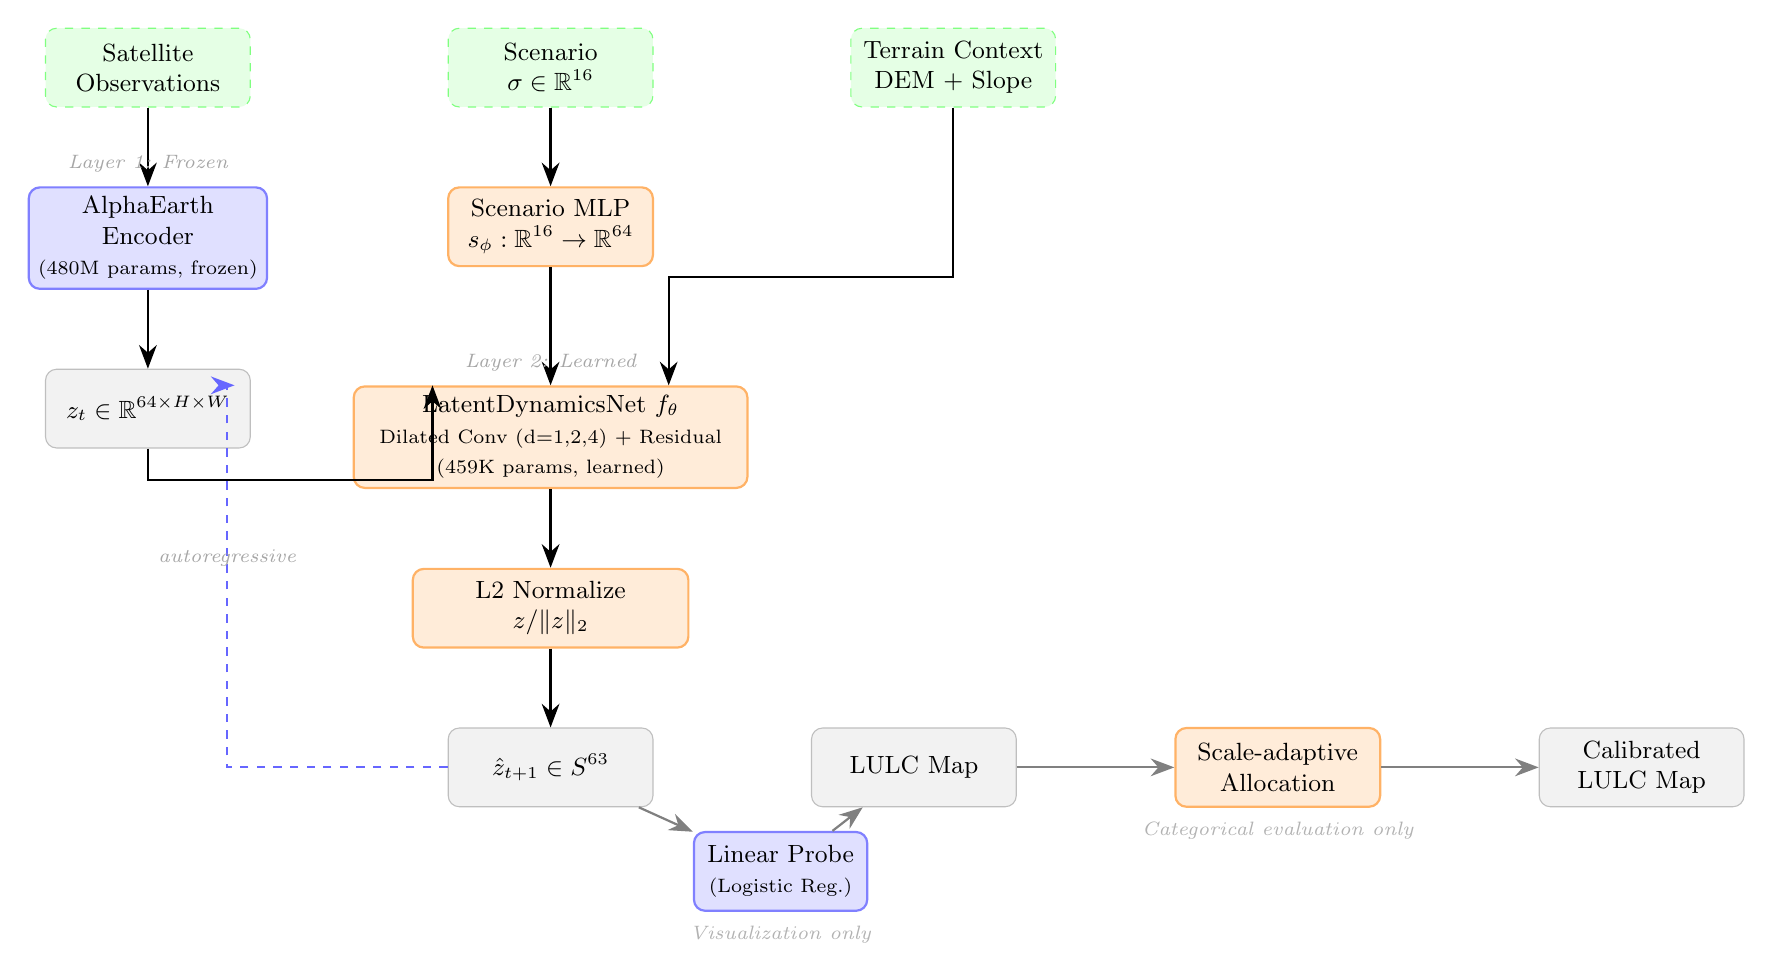
\begin{tikzpicture}[
    node distance=1.2cm and 1.8cm,
    box/.style={draw, rounded corners, minimum height=1.0cm, minimum width=2.6cm, align=center, font=\small},
    frozen/.style={box, fill=blue!12, draw=blue!50, thick},
    learned/.style={box, fill=orange!15, draw=orange!60, thick},
    input/.style={box, fill=green!10, draw=green!50, dashed},
    output/.style={box, fill=gray!10, draw=gray!50},
    arr/.style={-{Stealth[length=3mm]}, thick},
    label/.style={font=\scriptsize\itshape, text=gray!70},
]

% Row 1: Inputs
\node[input] (sat) {Satellite\\Observations};
\node[input, right=2.5cm of sat] (scenario) {Scenario\\$\sigma \in \mathbb{R}^{16}$};
\node[input, right=2.5cm of scenario] (terrain) {Terrain Context\\DEM + Slope};

% Row 2: Encoder + Scenario MLP
\node[frozen, below=1.0cm of sat] (encoder) {AlphaEarth\\Encoder\\{\scriptsize(480M params, frozen)}};
\node[learned, below=1.0cm of scenario] (smlp) {Scenario MLP\\$s_\phi: \mathbb{R}^{16} \to \mathbb{R}^{64}$};

% Row 3: Embedding
\node[output, below=1.0cm of encoder] (zt) {$z_t \in \mathbb{R}^{64 \times H \times W}$};

% Row 4: Dynamics
\node[learned, below=1.5cm of smlp, minimum width=5cm] (dynamics) {LatentDynamicsNet $f_\theta$\\{\scriptsize Dilated Conv (d=1,2,4) + Residual}\\{\scriptsize (459K params, learned)}};

% Row 5: Normalize
\node[learned, below=1.0cm of dynamics, minimum width=3.5cm] (norm) {L2 Normalize\\$z / \|z\|_2$};

% Row 6: Output + Decoder
\node[output, below=1.0cm of norm] (ztp1) {$\hat{z}_{t+1} \in S^{63}$};
\node[output, right=2.0cm of ztp1] (lulc) {LULC Map};
\node[learned, right=2.0cm of lulc, minimum width=2.6cm] (allocation) {Scale-adaptive\\Allocation};
\node[output, right=2.0cm of allocation] (calibrated) {Calibrated\\LULC Map};

% Decoder
\node[frozen, below right=0.3cm and 0.5cm of ztp1, minimum width=2.2cm] (decoder) {Linear Probe\\{\scriptsize(Logistic Reg.)}};

% Arrows: inputs to processing
\draw[arr] (sat) -- (encoder);
\draw[arr] (encoder) -- (zt);
\draw[arr] (scenario) -- (smlp);

% Concat arrows into dynamics
\draw[arr] (zt.south) -- ++(0,-0.4) -| ([xshift=-1.5cm]dynamics.north);
\draw[arr] (smlp.south) -- ([xshift=0cm]dynamics.north);
\draw[arr] (terrain.south) -- ++(0,-2.15) -| ([xshift=1.5cm]dynamics.north);

% Dynamics to normalize
\draw[arr] (dynamics) -- (norm);

% Normalize to output
\draw[arr] (norm) -- (ztp1);

% Autoregressive loop
\draw[arr, dashed, blue!60] (ztp1.west) -- ++(-2.8,0) |- ([xshift=-1.5cm]dynamics.north west) node[pos=0.25, above, label] {autoregressive};

% Decoder path
\draw[arr, gray] (ztp1) -- (decoder);
\draw[arr, gray] (decoder) -- (lulc);
\draw[arr, gray] (lulc) -- (allocation);
\draw[arr, gray] (allocation) -- (calibrated);

% Labels
\node[label, above=0.05cm of encoder] {Layer 1: Frozen};
\node[label, above=0.05cm of dynamics] {Layer 2: Learned};
\node[label, below=0.05cm of decoder, text=gray!60] {Visualization only};
\node[label, below=0.05cm of allocation, text=gray!60] {Categorical evaluation only};

\end{tikzpicture}
}
\caption{Architecture. The core \textbf{GeoFM-LDN} components are the frozen AlphaEarth encoder (blue) and the LatentDynamicsNet (orange, learned) that predicts residual state transitions in embedding space with explicit L2 re-normalization after each step. The dashed blue arrow represents the autoregressive feedback loop during multi-step rollout. The right-hand grey path is used only for evaluation: a linear probe decoder produces categorical LULC maps, and the optional \textbf{SA-Alloc} module then re-calibrates the change-pixel count for controlled comparison against cellular-automata allocators. \textbf{Scenario inputs are a reserved architectural interface, not an evaluated feature of this paper}: the scenario MLP is drawn dashed and is held constant at the baseline index during all reported experiments. Section~\ref{sec:limitations_scenario} explains why we do not present scenario-conditioned counterfactual results and what would be required to activate them.}
\label{fig:architecture}
\end{figure}

\subsection{LatentDynamicsNet}
\label{sec:network}

The dynamics model predicts the residual change in embedding space:
\begin{equation}
\hat{z}_{t+1} = \text{normalize}\Big(z_t + f_\theta\big([z_t \,\|\, s_\phi(\sigma) \,\|\, c]\big)\Big)
\label{eq:dynamics}
\end{equation}
where $z_t \in \mathbb{R}^{64 \times H \times W}$ is the current embedding grid, $\sigma \in \mathbb{R}^{16}$ is the scenario encoding, $s_\phi: \mathbb{R}^{16} \to \mathbb{R}^{64}$ is a two-layer MLP that maps the scenario to embedding dimension and broadcasts spatially, $c \in \mathbb{R}^{2 \times H \times W}$ is the terrain context (DEM elevation + slope), and $\text{normalize}(\cdot)$ denotes L2 normalization along the channel dimension.

The dynamics function $f_\theta$ is a dilated convolutional network:
\begin{equation}
\begin{aligned}
f_\theta ={}& \text{Conv}_{1\times1}^{128 \to 64} \circ \text{GN-GELU}
\circ \text{DilConv}_{3\times3}^{d=4} \circ \text{GN-GELU} \\
& \circ \text{DilConv}_{3\times3}^{d=2} \circ \text{GN-GELU}
\circ \text{DilConv}_{3\times3}^{d=1}.
\end{aligned}
\end{equation}
where DilConv denotes dilated convolution with the specified dilation rate, and GN-GELU denotes GroupNorm (8 groups) followed by GELU activation. The input to the first layer has $64 + 64 + 2 = 130$ channels (embedding + scenario + terrain context). Dilation rates of 1, 2, 4 yield a theoretical receptive field of 17$\times$17 pixels (170\,m at 10\,m resolution), allowing local context to include features such as road construction edges or urban expansion fronts.

\textbf{Design rationale.} (1) \textit{Residual connection}: inter-annual embedding change is small (cosine similarity $\approx$0.96); learning the residual $\Delta z = f_\theta(\cdot)$ rather than the absolute $z_{t+1}$ avoids the identity-mapping collapse. (2) \textit{GroupNorm}: with the tabular development split of 12 training areas $\times$ 7 annual pairs (2017--2024), only 84 area-year pairs are available for supervised training, further reduced to $\approx$60 after excluding pairs with missing cache; BatchNorm statistics on such a small stream are unreliable, and GroupNorm is batch-size invariant. (3) \textit{L2 normalisation}: AlphaEarth embeddings lie on the 64-dimensional unit hypersphere; without explicit re-projection after residual addition, the embeddings drift off-manifold, causing downstream decoder failure (Section~\ref{sec:manifold}). The small training-sample regime is a plausible contributor to the negative expanded paired-inference result in Section~\ref{sec:results}; increasing the training-area count remains a first-order improvement.

\subsection{Baseline dynamics and scenario placeholder}
\label{sec:limitations_scenario}

The architecture includes a scenario encoding vector $\sigma \in \mathbb{R}^{16}$ so that future versions can condition dynamics on policy or environmental drivers. In the experiments reported here, however, all observed historical transitions are treated as the baseline trajectory, and the scenario input is fixed to the baseline index for the entirety of training and evaluation. In Eq.~\ref{eq:dynamics} below, $s_\phi(\sigma)$ is therefore a constant broadcast tensor for every reported result; the scenario branch does not contribute any learnable variation in the empirical results and should be read as a reserved architectural interface only.

\textbf{Scope of the present model.} The current model is a \textit{baseline-trend predictor} in the embedding space of a frozen encoder. We do not report counterfactual policy-scenario results, because non-baseline scenario weights have not received direct supervision. Activating scenario-conditioned counterfactual simulation would require one of: (a) scenario-labelled historical interventions (e.g., regions with documented Grain-for-Green implementation windows), (b) policy-specific hard constraints on decoded outputs, or (c) another source of supervised counterfactual signal. We treat this as a first-order limitation and list it explicitly in Section~\ref{sec:limitations}.

\begin{table}[htbp]
\centering
\caption{Scenario indices reserved by the architecture. Only the baseline input is trained and evaluated in this study.}
\label{tab:scenarios}
\small
\begin{tabular}{clp{0.55\textwidth}}
\toprule
ID & Name & Description \\
\midrule
0 & Urban sprawl & Reserved; not evaluated here \\
1 & Ecological restoration & Reserved; not evaluated here \\
2 & Agricultural intensification & Reserved; not evaluated here \\
3 & Climate adaptation & Reserved; not evaluated here \\
4 & Baseline & Historical trend continuation; trained and evaluated \\
\bottomrule
\end{tabular}
\end{table}

\subsection{Manifold preservation via L2 normalization}
\label{sec:manifold}

AlphaEarth embeddings are L2-normalized unit vectors. The residual operation $z + \Delta z$ does not preserve unit norm. Over $k$ autoregressive steps, the embedding norm diverges as $\|z_k\| \neq 1$, causing the downstream linear decoder (trained on unit vectors) to encounter out-of-distribution inputs.

We enforce manifold preservation by re-normalizing after each step:
\begin{equation}
z_{t+1} = \frac{z_t + f_\theta(z_t, s, c)}{\|z_t + f_\theta(z_t, s, c)\|_2}
\end{equation}

We verify empirically that after 20 autoregressive steps, all pixel vectors maintain $\|z\|_2 = 1.0$ with error $<10^{-5}$.

\subsection{Multi-step unrolled training}
\label{sec:multistep}

Standard single-step training (teacher forcing) creates exposure bias: the model is trained with ground-truth inputs but at inference must consume its own predictions. To mitigate this, we unroll the autoregressive loop for $K=3$ steps during training and compute a weighted sum of losses:
\begin{equation}
\mathcal{L} = \sum_{k=1}^{K} \frac{1}{2^{k-1}} \|\hat{z}_{t+k} - z_{t+k}\|_2^2
\end{equation}
where $\hat{z}_{t+k}$ is the $k$-step predicted embedding (each step using the previous prediction as input) and $z_{t+k}$ is the ground truth. The exponentially decaying weights prioritize short-term accuracy while still encouraging long-horizon consistency.

\subsection{LULC decoder}

Predicted embeddings can be decoded to LULC classes for visualisation using a linear probe (scikit-learn LogisticRegression, max\_iter=1000). The probe is trained on 2020 AlphaEarth embeddings paired with ESRI Global LULC labels. A traceable 5-fold cross-validation run over \textbf{six ESRI class codes} (merged from the raw nine, see below) gives 76.99\% overall accuracy over 5{,}119 samples. This decoder is not used for dynamics training.

\paragraph{ESRI 9-class $\to$ 6-class merge rule.} The raw ESRI Global LULC 10\,m Time Series distinguishes 9 classes: water, trees, flooded vegetation, crops, built area, bare ground, snow/ice, clouds, and rangeland. On our study areas, three classes are too sparse to fit a well-conditioned linear probe: flooded vegetation appears in only Poyang Lake, snow/ice appears only in Qinghai Edge and Daxinganling, and clouds appear as a residual class rather than a genuine land-cover state. We merge as follows: (i) flooded vegetation is folded into water; (ii) snow/ice and bare ground are merged into ``bare/snow''; (iii) clouds are dropped. This yields six operational classes: water, trees, crops, built area, bare/snow, and rangeland. The merge is applied uniformly to training labels, validation labels, and the transition-prior baseline. The mapping is released as a JSON manifest in the public repository and is applied identically to every method compared in Section~\ref{sec:independent_change_validation} and Section~\ref{sec:geosos_flus_results}.

\paragraph{Decoder time stability.} The original decoder was trained only on 2020 embeddings. To test decoder year-drift, we retrain annual logistic-regression decoders for 2017--2024 and re-decode every validation pair whose predicted-embedding grid matches the reference label grid (Section~\ref{sec:peryear_decoder}). This analysis improves end-year categorical accuracy on 8/9 re-evaluable pairs, but two Banzhucun multi-year windows remain excluded because their predicted-embedding grids do not match the label grids.

\subsection{Scale-adaptive spatial-demand allocation (SA-Alloc)}
\label{sec:scale_adaptive_allocation}

Decoded LULC maps from GeoFM-LDN can over-predict change area, especially when the candidate region is much larger than the calibration townships. To make categorical comparisons more conservative and reproducible, we apply an optional post-processor called SA-Alloc. \textbf{SA-Alloc is not part of GeoFM-LDN's forward model} and is not used during embedding training. It only converts the decoded baseline-trend prediction into a calibrated categorical map for metrics such as change F1, figure of merit (FoM), transition accuracy, and allocation disagreement, and is the module used in the same-grid GeoSOS-FLUS ablation of Section~\ref{sec:geosos_flus_results}.

For each target area, candidate change pixels are those where the decoded prediction differs from the start-year reference map. Let $p_c$ be the candidate change fraction and let $p^\ast$ be the calibrated target change fraction. We estimate a ratio model from calibration areas:
\begin{equation}
p^\ast = \mathrm{clip}\left(p_c \, r_q \, m(A),\, p_{\min},\, p_{\max}\right),
\end{equation}
where $r_q$ is the $q=0.25$ quantile of observed-to-candidate change ratios in the calibration set, $p_{\min}=0.05$, $p_{\max}=0.25$, and $m(A)$ is a scale-dependent multiplier. The final calibrated configuration uses $m(A)=1.5$ for regions with fewer than 50{,}000 valid pixels and $m(A)=3.0$ otherwise. This rule preserves the calibrated small-region behavior observed on the 24-township benchmark while allowing larger external validation regions to keep enough candidate changes to avoid systematic under-prediction.

The allocation gate then ranks candidate change pixels using the change score, multi-scale class-aligned neighborhood support, and transition reliability estimated from held-out calibration labels. The final score adds target-neighborhood support with weight 1.5, subtracts source-neighborhood support with weight 0.65, and adds transition-reliability support with weight 0.6 across neighborhood windows of 3, 5, and 9 pixels. The highest-ranked candidates are retained until the target change budget is reached; all other candidate pixels revert to the start-year class. The manifest for each run records the valid-pixel count, selected multiplier, target change fraction, and retained change pixels, making the allocation step traceable.

\paragraph{Hand-tuned constants and their status.} SA-Alloc contains eleven hand-tuned constants: the small-region multiplier (1.5), the large-region multiplier (3.0), the valid-pixel threshold separating them (50{,}000), the change-fraction floor ($p_{\min}=0.05$), the change-fraction ceiling ($p_{\max}=0.25$), the quantile used to estimate $r_q$ ($q=0.25$), the target-neighborhood weight (+1.5), the source-neighborhood weight ($-0.65$), the transition-reliability weight (+0.6), and the three neighborhood window sizes (3, 5, 9). These were fit by inspection on the 24-township benchmark and were \emph{not} re-tuned when the four external validation regions were added. We view them as an empirically calibrated configuration, not as universal geographic constants, and we did not run a full sensitivity sweep. A short discussion of the practical risk this introduces is deferred to Section~\ref{sec:limitations} (limitation~\ref{lim:magic_numbers}).

\subsection{Inference procedure}

Given a bounding box and prediction horizon $N$:
\begin{enumerate}
\item Extract year-$t$ AlphaEarth embeddings from GEE.
\item Optionally extract DEM/slope terrain context.
\item Encode the baseline trajectory as a 16-dimensional vector.
\item Autoregressive loop: for $k = 1, \ldots, N$, compute $z_{t+k}$ via Eq.~\ref{eq:dynamics} with L2 normalization.
\item Optionally decode $z_{t+k}$ to LULC classes for visualization; quantitative dynamics evaluation remains in embedding space.
\end{enumerate}


% ============================================================================
\section{Experiments}
\label{sec:experiments}
% ============================================================================

\subsection{Experimental setup}

\textbf{Data splits.} The development workflow used 12 training areas, 2 validation areas, 1 test area, and 2 out-of-distribution areas. Gridded cached embeddings support the convolutional dynamics model, while point-sampled embeddings are used only for lightweight feasibility and diagnostic checks. In the revised data-traceable summary, area-level statistics are reported only for cached grids with valid non-placeholder metrics.

\textbf{Training.} Adam optimizer ($\text{lr} = 10^{-3}$), 100 epochs, 3-step unrolled loss with decaying weights $[1.0, 0.5, 0.25]$. Training completes in $\approx$80\,s on CPU (Intel i7-12700). No GPU required.

\textbf{Metrics.} (1) Cosine similarity between predicted and ground-truth embeddings (primary metric). (2) Mean squared error (MSE). (3) L2 distance. All metrics are computed per-pixel and averaged.

\subsection{Baseline methods}

\begin{itemize}
\item \textbf{Persistence:} $\hat{z}_{t+1} = z_t$ (``next year equals this year'')---the standard naive baseline in time-series forecasting.
\item \textbf{Linear extrapolation:} $\hat{z}_{t+1} = 2z_t - z_{t-1}$ (linear trend continuation).
\item \textbf{Label-only transition prior:} for categorical validation only, we estimate empirical start-class to end-class transition frequencies from other available ESRI label pairs with the same grid shape and apply those frequencies to the target start-year map. This baseline uses no AlphaEarth embeddings and no LatentDynamicsNet prediction, so it tests whether apparent change detection is explained only by coarse class-transition frequencies.
\end{itemize}

\subsection{Change-pixel evaluation protocol}

Global cosine similarity is dominated by pixels with weak annual embedding displacement. To diagnose whether the model captures localized dynamics rather than only predicting stasis, we stratify evaluation:
\begin{itemize}
\item \textbf{Changed pixels:} top 20\% by L2 distance between $z_t$ and $z_{t+1}$ (embedding-displacement proxy).
\item \textbf{Stable pixels:} bottom 20\% by the same distance.
\end{itemize}
This diagnostic tests whether the model captures representation dynamics or merely predicts stasis; it is not a substitute for independent labelled land-cover change validation.

\subsection{Independent categorical change-validation protocol}
\label{sec:independent_change_protocol}

To convert the embedding-displacement diagnostic into a formal land-cover transition test, we implemented a separate validation protocol that operates on annual categorical LULC maps. The protocol requires three co-registered arrays for each area--year pair: the reference start-year map $y_t$, the reference end-year map $y_{t+1}$, and the decoded model prediction $\hat{y}_{t+1}$. Reference labels and predicted maps are stored under \path{data/independent_change_labels/labels} and \path{data/independent_change_labels/predicted}, respectively, using area and year identifiers in the filenames. A persistence baseline is computed internally as $\hat{y}_{t+1}=y_t$.

The validation script reports binary change precision, recall, and F1; end-year categorical accuracy; accuracy on truly changed pixels; exact transition-match accuracy on changed pixels; and class-area bias measured as the mean absolute difference between predicted and reference class fractions. We include two controls beyond persistence. First, a spatially shuffled model negative control randomly permutes the predicted end-year map with a fixed seed, preserving the predicted class histogram while destroying spatial correspondence. This control tests whether the decoded dynamics carry spatially localized transition information rather than only predicting plausible class proportions. Second, a label-only transition prior estimates empirical categorical transition frequencies from other available ESRI label pairs and applies those frequencies to the target start-year map without using embeddings or model predictions. This tests whether the model's change signal is stronger than a simple categorical transition-frequency prior. The script writes per-area CSV rows and transition-count tables. The released validation set contains 12 completed independent area--year pairs across Banzhucun, Bishan, Heping, Poyang Lake, and Wuyi Mountain, with no skipped label--prediction pairs in the current cache.

\subsection{Same-grid GeoSOS-FLUS comparison protocol}
\label{sec:geosos_flus_protocol}

We further compare GeoFM-LDN (with and without SA-Alloc) against the GeoSOS-FLUS console implementation under a controlled same-grid protocol. The comparison isolates the final categorical allocation problem rather than attempting a full native GeoSOS-FLUS deployment. Both methods operate on the same start-year map, label grid, and target evaluation mask, and GeoSOS-FLUS is configured from prediction-side suitability and demand information rather than from target end-year truth. This design avoids giving the cellular-automata baseline access to reference change while keeping the evaluation grid identical. It should not be read as a production GeoSOS-FLUS experiment with locally calibrated ANN drivers and full socioeconomic or biophysical covariates. Accordingly, the primary evidence for this ablation is the per-area win/loss matrix in Table~\ref{tab:flus_per_area_wins}, not aggregate means.

Two validation groups are used. The first is the original 24-township same-grid benchmark, which contains township-scale samples with 3,176--37,126 valid pixels. The second contains four larger external regions (Dongguan, Kunshan, Anxin, and Caidian) with 50,634--421,812 valid pixels. The scale-adaptive allocation rule described in Section~\ref{sec:scale_adaptive_allocation} therefore uses the small-region multiplier for all 24 township samples and the large-region multiplier for all four external samples. For each group, we report mean change F1, FoM, transition accuracy on true changed pixels, and allocation disagreement. We also run five GeoSOS-FLUS random seeds (1001--1005) and summarize overall mean deltas relative to GeoSOS-FLUS.

\subsection{Empirical evidence chain and validation boundary}
\label{sec:evidence_chain}

To make the empirical workflow transparent, we summarize the evidence chain that links each analysis stage to the claim it can support. The classification distinguishes results that directly support the main embedding-space claim from diagnostic probes that support bounded interpretation but not standalone operational claims. Table~\ref{tab:empirical_pipeline} is therefore part of the empirical design rather than a post hoc disclaimer.

\begin{table}[htbp]
\centering
\caption{Empirical evidence chain and validation boundary. Complete stages directly support manuscript claims; diagnostic stages support interpretation or application probing only.}
\label{tab:empirical_pipeline}
\scriptsize
\setlength{\tabcolsep}{2pt}
\renewcommand{\arraystretch}{0.92}
\begin{tabular}{@{}P{0.20\textwidth}P{0.11\textwidth}P{0.37\textwidth}P{0.26\textwidth}@{}}
\toprule
Empirical stage & Status & Evidence in this manuscript & Boundary / next validation \\
\midrule
Area-level embedding dynamics & No clear advantage & 30 complete 2017--2024 areas; aligned-cache LDN mean advantage $-0.0030$; 16/30 positive; Wilcoxon $p=0.57$. & Does not beat persistence; cache--checkpoint alignment is required. \\
Encoder replacement ablation & Diagnostic & Prithvi-100M CLS branch on 17 areas; mean advantage $-2.4\times 10^{-6}$; CLS is nearly stationary. & State-resolution diagnostic, not an encoder-size benchmark. \\
Semantic decoder validation & Diagnostic & 5,119 AlphaEarth--ESRI samples; six classes; 2020 CV accuracy 76.99\%; per-year decoders add 0.0778 over nine pairs. & Decoder drift is real; improved decoding does not establish full-map forecasting skill. \\
Planning feature dropout & Diagnostic & 45 policies; dropout 0.3 retains 86.8\% of full-feature slope improvement; embedding-only retains 12.9\%. & Single-county application probe, not operational planning deployment. \\
Embedding-space transfer probe & Weak signal & Banzhucun $\to$ Heping policy improves embedding-space reward by +5.5 vs. random and +13.1 vs. greedy. & One diagnostic reward system; decoded cropland-change delta is near neutral. \\
Independent change-label validation & Split verdict & 11 usable ESRI-label pairs: change F1 0.365 vs. shuffled 0.294 and transition prior 0.182; end-year accuracy 0.636 vs. persistence 0.832. & Change-screening signal only; not a full-map categorical forecaster. \\
Same-grid GeoSOS-FLUS ablation & Split verdict & 24 townships; best SA-Alloc variant wins change F1 13/11, FoM 11/13, transition accuracy 9/14, allocation disagreement 16/8. & Stripped-down FLUS console only; native-driver comparison remains future work. \\
\bottomrule
\end{tabular}
\renewcommand{\arraystretch}{1.0}
\end{table}


% ============================================================================
\section{Results}
\label{sec:results}
% ============================================================================

\subsection{Phase 0: Embedding feasibility}

Before training any dynamics model, we verified three prerequisites on 3 areas $\times$ 7 years $\times$ 500 points:

\begin{table}[htbp]
\centering
\caption{Phase 0 feasibility validation results.}
\label{tab:phase0}
\begin{tabular}{lccc}
\toprule
Criterion & Threshold (pass/strong) & Result & Verdict \\
\midrule
Interannual cos.~sim. & $<$0.99 / $<$0.95 & 0.953 & PASS \\
Change/stable separation & $>$2$\times$ / $>$5$\times$ & 2.44$\times$ & PASS \\
Linear decode accuracy & $>$50\% / $>$70\% & 76.99\% & STRONG \\
\bottomrule
\end{tabular}
\end{table}

\subsection{Aggregate results and paired inference}

\begin{table}[htbp]
\centering
\caption{Data-traceable area-level prediction quality from 30 study areas with complete 2017--2024 time series (2023--2024 transition, refreshed embeddings). Persistence is per-pixel cosine similarity between 2023 and 2024 embeddings; Model is cosine similarity between predicted and observed 2024 embeddings.}
\label{tab:aggregate}
\begin{tabular}{lccc}
\toprule
Metric & $n$ areas & Mean & Range \\
\midrule
Persistence & 30 & 0.9652 & [0.9122, 0.9932] \\
LatentDynamicsNet & 30 & 0.9622 & [0.8950, 0.9856] \\
Model $-$ persistence & 30 & \textbf{$-$0.0030} & \textbf{[$-$0.0982, +0.0266]} \\
\bottomrule
\end{tabular}
\end{table}

\begin{table}[htbp]
\centering
\caption{Rigorous paired inference on Model $-$ Persistence over 30 complete-time-series study areas (refreshed embedding cache, dynamics checkpoint retrained on the same cache). The paired effect is small and not statistically significant.}
\label{tab:paired_inference}
\small
\begin{tabular}{lc}
\toprule
Quantity & Value \\
\midrule
$n$ areas & 30 \\
Mean paired difference & $-3.004 \times 10^{-3}$ \\
Standard deviation & $2.274 \times 10^{-2}$ \\
Positive / negative areas & 16 / 14 \\
Wilcoxon signed-rank $p$ (two-sided) & 0.570 \\
Paired $t$-test $p$ (two-sided) & 0.475 \\
Sign-flip permutation $p$ (two-sided) & 0.530 \\
Bootstrap 95\% CI & [$-1.21\times10^{-2}$, $+3.72\times10^{-3}$] \\
Cohen's $d_z$ & $-0.132$ \\
\bottomrule
\end{tabular}
\end{table}

\textbf{Reading of the paired inference.} Under the expanded aligned-cache evaluation, the one-step evidence is near-zero and not significant. The mean 1-step cosine advantage is $-3.004\times10^{-3}$, with 16/30 areas showing positive advantage. Wilcoxon signed-rank, paired $t$-test, sign-flip permutation, and bootstrap inference all fail to reject a zero-centred advantage. We therefore \textbf{do not claim that GeoFM-LDN is better than persistence in embedding-space one-step forecasting}. The result also shows that cache and checkpoint versions must be aligned before evaluating frozen-encoder dynamics. All reported embedding-space results use freshly re-extracted embeddings and retrained checkpoints from the same cache.

\subsection{Per-area results}

\begin{table}[htbp]
\centering
\caption{Per-area 1-step prediction quality for 30 complete-time-series study areas (2023--2024 transition, refreshed embeddings). Sorted by advantage descending.}
\label{tab:perarea}
\small
\begin{tabular}{lccc}
\toprule
Area & Model & Persistence & Advantage \\
\midrule
Qinghai Edge & 0.9613 & 0.9347 & \textbf{+0.0266} \\
Ordos Desert Edge & 0.9566 & 0.9354 & \textbf{+0.0212} \\
North China Plain & 0.9735 & 0.9576 & \textbf{+0.0159} \\
Northeast Plain & 0.9772 & 0.9667 & \textbf{+0.0105} \\
Tarim Oasis & 0.9609 & 0.9535 & \textbf{+0.0074} \\
Yunnan Eco & 0.9412 & 0.9354 & \textbf{+0.0058} \\
Wuhan Outer Ring & 0.9795 & 0.9746 & \textbf{+0.0049} \\
Hetao & 0.9591 & 0.9543 & \textbf{+0.0048} \\
Jianghan Plain & 0.9304 & 0.9285 & \textbf{+0.0019} \\
Chengdu Plain & 0.9448 & 0.9429 & \textbf{+0.0018} \\
Wumeng Mountains & 0.9775 & 0.9760 & \textbf{+0.0015} \\
Yangtze Delta & 0.9856 & 0.9845 & \textbf{+0.0012} \\
Dongting Wetland & 0.9133 & 0.9123 & \textbf{+0.0011} \\
Suzhou Fringe & 0.9823 & 0.9814 & \textbf{+0.0009} \\
Pearl River & 0.9808 & 0.9805 & \textbf{+0.0004} \\
Qinling South Slope & 0.9849 & 0.9846 & \textbf{+0.0004} \\
Guanzhong & 0.9847 & 0.9847 & $-2.5\times10^{-5}$ \\
Daxinganling & 0.9492 & 0.9494 & $-$0.0001 \\
Jing-Jin-Ji & 0.9852 & 0.9856 & $-$0.0003 \\
Wuyi Mountain & 0.9845 & 0.9850 & $-$0.0006 \\
Erhai Lake Margin & 0.9795 & 0.9800 & $-$0.0006 \\
Banzhucun & 0.9703 & 0.9713 & $-$0.0011 \\
Minnan Coast & 0.9837 & 0.9857 & $-$0.0021 \\
Bishan & 0.9760 & 0.9781 & $-$0.0022 \\
Guizhou Karst & 0.9756 & 0.9786 & $-$0.0029 \\
Changbai Lower Belt & 0.9790 & 0.9848 & $-$0.0059 \\
Gobi Margin & 0.9577 & 0.9681 & $-$0.0103 \\
Poyang Lake & 0.9334 & 0.9449 & $-$0.0116 \\
Hainan Coastal & 0.9020 & 0.9624 & $-$0.0605 \\
Bohai Delta & 0.8950 & 0.9932 & $-$0.0982 \\
\bottomrule
\end{tabular}
\end{table}

The largest positive advantages occur in Qinghai Edge (+0.0266), Ordos Desert Edge (+0.0212), and North China Plain (+0.0159). The largest degradations occur in Bohai Delta ($-$0.0982), Hainan Coastal ($-$0.0605), and Poyang Lake ($-$0.0116). Retraining on the refreshed embeddings removes the systematic negative shift seen when the cache and checkpoint were mismatched, but the resulting per-area distribution is still mixed and outlier-sensitive rather than a stable win over persistence. For this reason, the main inference relies on the 30-area aligned-cache table rather than on the smaller diagnostic grouping below.


Table~\ref{tab:category_diagnostic} groups the 10-area diagnostic baseline by the study-area categories in Table~\ref{tab:areas}. This table is included only to show why small-sample category summaries are unstable: the expanded 30-area cache contains additional named regions that do not share the original split/category ledger. It is not used as a formal category-level test, and the main inference relies on the 30-area paired table above rather than category means from the smaller split ledger.

\begin{table}[htbp]
\centering
\caption{Diagnostic grouping of the 10-area baseline by study-area category. Should not be interpreted as a formal biome-level statistical test due to small sample sizes per category.}
\label{tab:category_diagnostic}
\small
\begin{tabular}{lccc}
\toprule
Category & Areas in baseline & Mean advantage & Positive / negative \\
\midrule
Urban & 3 & $-$0.0070 & 0 / 3 \\
Agriculture & 2 & $-$0.0050 & 1 / 1 \\
Wetland & 1 & $-$0.0043 & 0 / 1 \\
Plateau & 1 & +0.0072 & 1 / 0 \\
Mixed & 2 & $-$0.0104 & 0 / 2 \\
Forest & 1 & $-$0.0146 & 0 / 1 \\
\bottomrule
\end{tabular}
\end{table}

\subsection{Per-year decoder retraining}
\label{sec:peryear_decoder}

The 2020-trained logistic-regression decoder may be mismatched when applied to predicted embeddings from other years. We therefore retrained separate decoders for each year from 2017 to 2024 and re-decoded every validation pair whose predicted-embedding grid matched the target label grid.

\begin{table}[htbp]
\centering
\caption{Per-year decoder cross-validation on ESRI labels. Accuracy and macro-F1 are computed by 5-fold cross-validation on the year-specific embedding--label samples available in the refreshed cache.}
\label{tab:decoder_by_year}
\small
\begin{tabular}{lccc}
\toprule
Year & $n$ samples & CV accuracy & Macro-F1 \\
\midrule
2017 & 800 & 0.6675 & 0.4935 \\
2018 & 800 & 0.7488 & 0.5139 \\
2019 & 800 & 0.7225 & 0.4881 \\
2020 & 24,967 & 0.8349 & 0.7352 \\
2021 & 24,969 & 0.8287 & 0.7056 \\
2022 & 800 & 0.7300 & 0.3856 \\
2023 & 800 & 0.7425 & 0.3999 \\
2024 & 800 & 0.7475 & 0.4617 \\
\bottomrule
\end{tabular}
\end{table}

Per-year decoder retraining improves end-year categorical accuracy by 0.0778 on average over nine re-evaluable pairs (median 0.0704, range $-0.0260$ to +0.1646), with 8/9 pairs improved. Two Banzhucun multi-year windows are excluded from this paired summary because their predicted-embedding grids are $8\times13$ while the reference label grids are $363\times610$. This result confirms that decoder year-drift contributed to the end-year accuracy gap. It does not, by itself, show that the dynamics model is a full-map forecaster, because even the retrained-decoder evaluation remains a decoded diagnostic downstream of the embedding-space prediction.

\subsection{Self-consistent embedding-displacement diagnostic}
\label{sec:embedding_displacement_diagnostic}

We report the top-20\% embedding-displacement diagnostic only as an internal consistency check. Defining ``changed'' pixels by high $\|z_{t+1}-z_t\|_2$ is nearly co-linear with the model's own training target, so evaluating the model on that subset is a form of self-consistent check rather than an independent land-cover change test. This diagnostic is therefore not used to support any independent change-detection claim.

\begin{table}[htbp]
\centering
\caption{Self-consistent embedding-displacement diagnostic on the single traceable cached region (Bishan). ``Advantage'' is model $-$ persistence cosine similarity on the top-20\% embedding-displacement pixels. Interpreted as an internal consistency check, not as a land-cover change validation.}
\label{tab:changepixel}
\begin{tabular}{lcccc}
\toprule
Area & Model & Persist. & Advantage & Source \\
\midrule
Bishan & 0.955710 & 0.955734 & $-2.35 \times 10^{-5}$ & cached grid \\
\bottomrule
\end{tabular}
\end{table}

The independent validation in Section~\ref{sec:independent_change_validation} therefore remains the only categorical transition test we report.

\subsection{Cosine similarity gap does not track end-year categorical accuracy}
\label{sec:cosine_to_accuracy}

Because the paired-inference tests in Table~\ref{tab:paired_inference} give a small effect size on cosine advantage while Section~\ref{sec:independent_change_validation} shows a 0.20 loss on end-year categorical accuracy, it is natural to ask whether per-area cosine advantage is even a useful predictor of per-area downstream accuracy. Table~\ref{tab:cosine_to_accuracy} joins the two per-area quantities on the areas where both are available.

\begin{table}[htbp]
\centering
\caption{Per-area cosine advantage over persistence versus per-area downstream end-year accuracy delta (model minus persistence) from the independent ESRI-label validation. Both areas where the two quantities can be joined are shown; a positive cosine advantage does not translate into a positive end-year accuracy delta.}
\label{tab:cosine_to_accuracy}
\small
\begin{tabular*}{\textwidth}{@{\extracolsep{\fill}}lcccc@{}}
\toprule
Area & Cosine advantage & Model end acc. & Persistence end acc. & $\Delta$ end acc. \\
\midrule
Bishan       & $-0.00622$ & 0.6405 & 0.8549 & $-0.2144$ \\
Poyang Lake  & $+0.01201$ & 0.7429 & 0.8261 & $-0.0832$ \\
\bottomrule
\end{tabular*}
\end{table}

Two areas is too small a sample for a formal correlation test, but the pattern is directly informative: on the L2-normalized unit hypersphere, a $\sim$1\% cosine similarity difference does not translate into a positive full-map end-year accuracy difference; both areas lose 8--21 percentage points relative to persistence. This is why we no longer treat cosine similarity as a headline metric for a categorical LULC forecaster: the metric compresses too much of the semantically important variation into a very narrow interval near 1.0. Cosine advantage is retained here as a representation-space diagnostic, not as a proxy for downstream deployment quality.

\subsection{Independent categorical change validation}
\label{sec:independent_change_validation}

We evaluated decoded model predictions against independently extracted ESRI Global LULC annual labels on 12 area--year pairs with matching cached prediction grids (Table~\ref{tab:independent_change_validation}). The evaluated set includes two Banzhucun three-year windows, seven annual Bishan windows, one Heping three-year window, and two held-out validation/test-area windows from Poyang Lake and Wuyi Mountain. Reference change rates range from 0.0\% in Wuyi Mountain 2020--2021 to 26.9\% in Banzhucun 2020--2023.

The Wuyi Mountain 2020--2021 pair has a reference change rate of 0.0\%, which makes binary change precision, recall, and F1 mathematically ill-defined for every method: any method that predicts even a single changed pixel receives $F1=0$ trivially, and any method that predicts zero changed pixels also receives $F1=0$ by the common $0/0 \to 0$ convention. Reporting Wuyi in the 12-pair mean therefore artificially deflates the model's mean and inflates the persistence baseline's apparent competence (a persistence F1 of $0$ on Wuyi does \emph{not} reflect an inability to detect change; the reference itself contains no change). All paired-inference statistics below are therefore computed on the 11 pairs with strictly positive reference change; the 12-pair mean is retained in Table~\ref{tab:independent_change_validation} for completeness. The raw pair-level values are released as \texttt{independent\_change\_validation\_by\_area.csv} in the public repository.

\begin{table}[htbp]
\centering
\caption{Independent categorical change validation against ESRI annual LULC labels. Change metrics treat a pixel as changed when the end-year class differs from the start-year class. The shuffled control randomly permutes the model-predicted end-year map, preserving predicted class frequencies while removing spatial correspondence. The transition-prior baseline uses empirical class-transition frequencies from other label pairs with the same grid shape and contains no embedding or model-prediction information. Persistence predicts the end-year map as identical to the start-year map.}
\label{tab:independent_change_validation}
\scriptsize
\setlength{\tabcolsep}{2pt}
\resizebox{\textwidth}{!}{%
\begin{tabular}{lcccccccc}
\toprule
Area--years & Chg. \% & Model F1 & Shuf. F1 & Prior F1 & Chg.-pix. acc. & Model end acc. & Prior end acc. & Pers. end acc. \\
\midrule
Banzhucun 2017--2020 & 22.1 & 0.371 & 0.335 & 0.226 & 0.303 & 0.535 & 0.667 & 0.779 \\
Banzhucun 2020--2023 & 26.9 & 0.482 & 0.417 & 0.297 & 0.292 & 0.558 & 0.656 & 0.731 \\
Bishan annual mean (7 pairs) & 14.5 & 0.344 & 0.254 & 0.177 & 0.342 & 0.641 & 0.749 & 0.855 \\
Heping 2017--2020 & 16.8 & 0.375 & 0.317 & 0.235 & 0.191 & 0.676 & 0.772 & 0.832 \\
Poyang Lake 2020--2021 & 17.4 & 0.385 & 0.389 & 0.000 & 0.163 & 0.743 & 0.826 & 0.826 \\
Wuyi Mountain 2020--2021 & 0.0 & 0.000 & 0.000 & 0.000 & 0.000 & 0.996 & 1.000 & 1.000 \\
\midrule
Mean (12 pairs) & 15.4 & 0.335 & 0.269 & 0.166 & 0.279 & 0.666 & 0.764 & 0.846 \\
\bottomrule
\end{tabular}
}
\end{table}

\begin{table}[htbp]
\centering
\caption{Paired inference on the independent categorical change validation, 11 area--year pairs (Wuyi Mountain 2020--2021 excluded). Each row compares the model prediction against a single control (higher is better for change F1, end-year accuracy, changed-pixel accuracy, and transition exact match; lower is better for area-bias MAE). The win/loss column follows the metric direction; for area-bias MAE, a win means lower model MAE. Wilcoxon and sign-test $p$-values are two-sided.}
\label{tab:independent_change_paired}
\scriptsize
\setlength{\tabcolsep}{2pt}
\resizebox{\textwidth}{!}{%
\begin{tabular}{@{}llcccccc@{}}
\toprule
Metric & Control & Model mean & Ctrl mean & Mean $\Delta$ & Wins/losses & Wilcoxon $p$ & Sign $p$ \\
\midrule
Change F1               & Shuffled model      & 0.365 & 0.294 & $+0.072$ & 10 / 1 & 0.002 & 0.012 \\
Change F1               & Transition prior    & 0.365 & 0.182 & $+0.184$ & 11 / 0 & 0.001 & 0.001 \\
Change F1               & Persistence         & 0.365 & 0.000 & $+0.365$ & 11 / 0 & 0.001 & 0.001 \\
End-year accuracy       & Persistence         & 0.636 & 0.832 & $-0.196$ & 0 / 11 & 0.001 & 0.001 \\
End-year accuracy       & Transition prior    & 0.636 & 0.742 & $-0.106$ & 0 / 11 & 0.001 & 0.001 \\
Changed-pixel accuracy  & Shuffled model      & 0.304 & 0.289 & $+0.016$ & 8 / 3 & 0.365 & 0.227 \\
Changed-pixel accuracy  & Transition prior    & 0.304 & 0.090 & $+0.214$ & 11 / 0 & 0.001 & 0.001 \\
Area-bias MAE (lower)   & Persistence         & 0.082 & 0.029 & $+0.053$ & 1 / 10 & 0.002 & 0.012 \\
Area-bias MAE (lower)   & Transition prior    & 0.082 & 0.026 & $+0.056$ & 1 / 10 & 0.002 & 0.012 \\
Transition exact match  & Transition prior    & 0.304 & 0.090 & $+0.214$ & 11 / 0 & 0.001 & 0.001 \\
\bottomrule
\end{tabular}}
\end{table}

The independent validation gives a \textbf{split verdict}:

\begin{itemize}
\item \textbf{On binary change detection}, the model beats the spatially shuffled model on change F1 in 10 of 11 pairs (Wilcoxon $p=0.002$) and beats the label-only transition prior in 11 of 11 pairs (Wilcoxon $p=0.001$). Persistence has F1$=0$ by construction on every pair because it predicts no change. These three pairwise gaps support a bounded claim: decoded GeoFM-LDN outputs carry \emph{some} spatially localized transition information above simple class-frequency priors.
\item \textbf{On full-map categorical accuracy}, the model loses to two baselines. End-year accuracy is 0.636 for the model vs.\ 0.832 for persistence (paired $\Delta = -0.196$, model loses 0 / 11) and 0.742 for the transition prior (paired $\Delta = -0.106$, model loses 0 / 11). Class-area MAE is 2.8$\times$ higher for the model (0.082 vs.\ 0.029 for persistence and 0.026 for the transition prior; model wins only 1 / 11 pairs).
\item \textbf{On changed-pixel accuracy}, the model shows only a small, non-significant advantage over the shuffled control ($\Delta=+0.016$, 8 wins / 3 losses, Wilcoxon $p=0.365$). Once we restrict attention to pixels that actually changed and ask ``did the model pick the right end class,'' spatial correspondence in the model's prediction is not clearly stronger than random spatial permutation of the same class histogram.
\end{itemize}

The evidence therefore supports the following claim, and no stronger claim: GeoFM-LDN's decoded output can serve as a \emph{change-detection screening layer}---it flags likely-changed pixels above two natural controls---but it is neither a full-map categorical forecaster (persistence and the transition prior are both better on end-year accuracy and class-area bias) nor a per-changed-pixel transition classifier (the shuffled control is not clearly beaten). Poyang Lake (the val-split area) is a case in point: model change F1 (0.385) is essentially tied with the shuffled control (0.389), and both are close to zero relative to the underlying label variability. The Wuyi Mountain 2020--2021 pair carries no signal in either direction and is excluded from the inferential analysis as discussed above.

\begin{figure}[htbp]
\centering
\includegraphics[width=\textwidth]{figures/fig_spatial_change_validation.pdf}
\caption{Spatial validation and failure-mode example for Banzhucun 2020--2023. Panels show the reference start-year map, reference end-year map, decoded model prediction, binary reference change, binary predicted change, and change-detection error classes. The model detects many true changed pixels (36,605 hits) but also produces substantial false alarms (55,763) and misses (22,983), illustrating why change F1 improves over controls while full-map categorical accuracy remains below persistence.}
\label{fig:spatial_change_validation}
\end{figure}

\subsection{Same-grid GeoSOS-FLUS allocation ablation}
\label{sec:geosos_flus_results}

We compare five candidate variants of GeoFM-LDN and GeoFM-LDN\,+\,SA-Alloc against the stripped-down GeoSOS-FLUS console on the 24-township benchmark under the controlled same-grid protocol of Section~\ref{sec:geosos_flus_protocol}. Aggregate mean deltas can overstate performance when township sizes differ, so we report the \textbf{per-area, per-metric win/loss matrix} together with sign-test and Wilcoxon signed-rank $p$-values. This unweighted evidence changes the interpretation substantially.

\begin{table}[htbp]
\centering
\caption{Per-area, per-metric win/loss of each GeoFM-LDN / SA-Alloc variant against the stripped-down GeoSOS-FLUS console on the 24 township grids ($n=24$). A ``win'' means the variant beats FLUS on that metric on that township (higher change F1, FoM, transition accuracy; lower allocation disagreement, marked with $\downarrow$). Sign-test and Wilcoxon signed-rank $p$-values are two-sided. Computed from the raw per-area metrics CSV released in the public repository.}
\label{tab:flus_per_area_wins}
\scriptsize
\setlength{\tabcolsep}{2pt}
\resizebox{\textwidth}{!}{%
\begin{tabular}{@{}llrrrrr@{}}
\toprule
Variant & Metric & Wins & Losses & Ties & Sign-test $p$ & Wilcoxon $p$ \\
\midrule
GeoFM-LDN (raw decoded) & Change F1               & 15 & 9  & 0 & 0.31 & 0.29 \\
GeoFM-LDN (raw decoded) & FoM                     & 7  & 17 & 0 & 0.06 & 0.29 \\
GeoFM-LDN (raw decoded) & Transition accuracy     & 22 & 0  & 2 & $<$0.001 & $<$0.001 \\
GeoFM-LDN (raw decoded) & Alloc.\ disag.$\downarrow$ & 2  & 22 & 0 & $<$0.001 & $<$0.001 \\
\midrule
+ Change-aware allocation gate & Change F1               & 13 & 11 & 0 & 0.84 & 0.39 \\
+ Change-aware allocation gate & FoM                     & 12 & 12 & 0 & 1.00 & 0.49 \\
+ Change-aware allocation gate & Transition accuracy     & 17 & 6  & 1 & 0.03 & 0.003 \\
+ Change-aware allocation gate & Alloc.\ disag.$\downarrow$ & 13 & 11 & 0 & 0.84 & 0.23 \\
\midrule
\textbf{SA-Alloc (external LOO)} & Change F1               & 12 & 12 & 0 & 1.00 & 0.28 \\
\textbf{SA-Alloc (external LOO)} & FoM                     & 11 & 13 & 0 & 0.84 & 0.86 \\
\textbf{SA-Alloc (external LOO)} & Transition accuracy     & 8  & 15 & 1 & 0.21 & 0.41 \\
\textbf{SA-Alloc (external LOO)} & Alloc.\ disag.$\downarrow$ & 16 & 8  & 0 & 0.15 & 0.24 \\
\midrule
\textbf{SA-Alloc + trans.\ floor 0.30} & Change F1               & 13 & 11 & 0 & 0.84 & 0.18 \\
\textbf{SA-Alloc + trans.\ floor 0.30} & FoM                     & 11 & 13 & 0 & 0.84 & 0.70 \\
\textbf{SA-Alloc + trans.\ floor 0.30} & Transition accuracy     & 9  & 14 & 1 & 0.40 & 0.92 \\
\textbf{SA-Alloc + trans.\ floor 0.30} & Alloc.\ disag.$\downarrow$ & 16 & 8  & 0 & 0.15 & 0.24 \\
\midrule
Regression hold-out cal.\ & Change F1               & 13 & 11 & 0 & 0.84 & 0.64 \\
Regression hold-out cal.\ & FoM                     & 10 & 14 & 0 & 0.54 & 0.29 \\
Regression hold-out cal.\ & Transition accuracy     & 11 & 13 & 0 & 0.84 & 0.62 \\
Regression hold-out cal.\ & Alloc.\ disag.$\downarrow$ & 14 & 10 & 0 & 0.54 & 0.58 \\
\bottomrule
\end{tabular}}
\end{table}

Three observations follow directly from Table~\ref{tab:flus_per_area_wins}.

\textbf{No variant dominates GeoSOS-FLUS on all four metrics.} The best case per metric is spread across variants: raw GeoFM-LDN wins transition accuracy 22 / 0 but loses allocation disagreement 2 / 22; the change-aware allocation gate wins transition accuracy 17 / 6 but is a wash on change F1 and FoM; the SA-Alloc external-LOO variants win allocation disagreement 16 / 8 and are near-tied on change F1 (12--13 / 11--12) but \emph{lose} FoM (11 / 13) and transition accuracy (8--9 / 14--15). Sign-test $p$-values for the four SA-Alloc metrics range from 0.15 to 1.00; none rejects the null of a fifty-fifty per-township outcome.

\textbf{The aggregate-mean result is driven by a small number of high-population townships.} Township valid-pixel counts range from 3{,}176 to 37{,}126, so pixel-weighted aggregate means over-represent the largest townships. Under a per-area, unweighted paired test---which is what a reader of a same-grid comparison would expect---the best aggregate variant produces roughly a coin flip on three of four metrics. We consider this the strictly more transparent way to report the ablation.

\textbf{The comparison is a controlled allocation ablation, not a native-driver competition.} The GeoSOS-FLUS console is here driven by prediction-derived suitability and demand rather than by locally calibrated ANN drivers and socioeconomic covariates. That constraint applies uniformly to every row above; it is not an advantage for GeoFM-LDN. But the result should not be read as a general or same-grid superiority claim for GeoFM-LDN: on three of the four metrics the per-area verdict is roughly a coin flip, and on transition accuracy the SA-Alloc variants actually lose. See Section~\ref{sec:limitations} (limitation~\ref{lim:flus_scope}) for the associated scope caveat.

The aggregate-mean table is included as secondary context in Table~\ref{tab:geosos_flus_same_grid_aggregate}; the reader should treat Table~\ref{tab:flus_per_area_wins} as the primary evidence.

\begin{table}[htbp]
\centering
\caption{Aggregate-mean same-grid comparison (secondary context only; the per-area paired-inference table above is the primary evidence). Township valid-pixel counts range from 3{,}176 to 37{,}126, so pixel-weighted aggregate means differ from unweighted per-area means.}
\label{tab:geosos_flus_same_grid_aggregate}
\scriptsize
\resizebox{\textwidth}{!}{%
\begin{tabular}{@{}llccccc@{}}
\toprule
Validation group & Method & $n$ & Change F1 & FoM & Trans. acc. & Alloc. disag. \\
\midrule
24 townships & GeoSOS-FLUS console                    & 24 & 0.263 & 0.120 & 0.281 & 0.060 \\
24 townships & GeoFM-LDN + SA-Alloc (floor 0.30)     & 24 & 0.288 & 0.125 & 0.286 & 0.058 \\
\bottomrule
\end{tabular}}
\end{table}

The five-seed GeoSOS-FLUS randomisation gave aggregate mean deltas that were positive for change F1, FoM, and transition accuracy and negative (i.e., improvement) for allocation disagreement, with 5/5 overall seed-level ``wins' in both the 24-township and external-region groups. Given the per-area verdict in Table~\ref{tab:flus_per_area_wins}, we interpret this as ``the aggregate mean is stable under FLUS randomisation,' not as ``every area is a win.' The full per-seed metric bundle is released in the public repository.

\subsection{Aligned-cache multi-step degradation diagnostic}

Table~\ref{tab:multistep} reports the corrected 6-step autoregressive rollout across all 30 complete-time-series AlphaEarth areas using the aligned-cache dynamics checkpoint. Persistence at step $k$ compares the previous true year $z_{t+k-1}$ with the target true year $z_{t+k}$, rather than comparing the initial state $z_t$ with every later target. The run therefore aligns the embedding cache and the dynamics checkpoint.

\begin{table}[htbp]
\centering
\caption{Corrected multi-step rollout over 30 complete-time-series AlphaEarth areas using the aligned refreshed embedding cache. Values are means over areas. Positive/negative counts refer to Model $-$ Persistence advantage for that step.}
\label{tab:multistep}
\small
\begin{tabular}{lcccc}
\toprule
Step & Persistence & Model & Advantage & Positive / negative \\
\midrule
1 & 0.9681 & 0.9642 & $-$0.0039 & 13 / 17 \\
2 & 0.9676 & 0.9509 & $-$0.0167 & 8 / 22 \\
3 & 0.9647 & 0.9322 & $-$0.0326 & 2 / 28 \\
4 & 0.9625 & 0.9190 & $-$0.0436 & 2 / 28 \\
5 & 0.9616 & 0.9089 & $-$0.0527 & 0 / 30 \\
6 & 0.9657 & 0.9028 & $-$0.0629 & 1 / 29 \\
\bottomrule
\end{tabular}
\end{table}

Both persistence and model similarity degrade with longer horizons, and the model degrades faster than persistence after the first step. Step 1 remains near zero and non-significant (mean advantage $-0.0039$, 13/30 positive, Wilcoxon $p=0.49$), matching the aligned one-step verdict above. From step 2 onward, however, the rollout advantage is significantly negative and worsens gradually, reaching $-0.0629$ at step 6 (1/30 positive; Wilcoxon $p=5.59\times10^{-9}$). The multi-step result therefore does not provide long-horizon evidence that GeoFM-LDN beats persistence, under the aligned checkpoint--embedding evaluation.

\subsection{Development scaling diagnostic: 2 vs.~12 training areas}
\label{sec:ablation_data}

\begin{table}[htbp]
\centering
\caption{Development diagnostic on the effect of training data scale. These values are retained as recorded run diagnostics and are not the primary data-traceable evidence.}
\label{tab:scaling}
\begin{tabular}{lcccc}
\toprule
 & \multicolumn{2}{c}{2 areas (Phase 1)} & \multicolumn{2}{c}{12 areas (Phase 2)} \\
\cmidrule(lr){2-3}\cmidrule(lr){4-5}
Metric & Train adv. & OOD gap & Train adv. & OOD gap \\
\midrule
Global cos.~sim. & +0.003 & $-$0.195 & \textbf{+0.012} & $\mathbf{-}$\textbf{0.012} \\
Train win rate & 50\% & --- & \textbf{100\%} & --- \\
\bottomrule
\end{tabular}
\end{table}

The recorded scaling diagnostic is consistent with the interpretation that training-area diversity matters for embedding-space dynamics. Because the revised area-level summary uses only valid cached grids, these scaling numbers are treated as supporting diagnostics rather than the main evidence.

\subsection{Development ablation diagnostic}
\label{sec:ablation}

To diagnose the role of each architectural component during model development, three ablated variants were trained on the same development split. Each variant removes exactly one component while keeping all others unchanged. Because the main analysis prioritizes cached-grid summaries with explicit source files, this table is treated as a development diagnostic rather than as the main statistical evidence.

\begin{table}[htbp]
\centering
\caption{Development ablation diagnostic. ``Advantage'' is model cosine similarity minus persistence baseline, averaged across the recorded development split. ``Change Adv.'' is computed on the top-20\% embedding-displacement pixels only.}
\label{tab:ablation}
\begin{tabular}{lccc}
\toprule
Variant & Train Adv. & Val Adv. & Change Adv. \\
\midrule
Full model & \textbf{+0.0135} & \textbf{+0.0019} & \textbf{+0.0290} \\
w/o L2 normalization & +0.0052 ($-$62\%) & $-$0.0021 & +0.0133 ($-$54\%) \\
w/o dilated conv. & +0.0102 ($-$24\%) & +0.0064 & +0.0197 ($-$32\%) \\
w/o unrolled loss ($K$=1) & +0.0120 ($-$11\%) & $-$0.0006 & +0.0295 \\
\bottomrule
\end{tabular}
\end{table}

\textbf{L2 normalization is the clearest development signal.} Removing it degrades the recorded training advantage by 62\% and causes the validation set to turn negative. This supports the design choice to re-project residual predictions onto the unit hypersphere after each step.

\textbf{Dilated convolutions primarily affect change-pixel diagnostics.} Replacing dilated convolutions (dilation rates 1, 2, 4; receptive field 170\,m) with standard 3$\times$3 convolutions (receptive field 50\,m) reduces the recorded change-pixel advantage by 32\% ($+0.029 \to +0.020$), while global metrics degrade by 24\%. This is consistent with expanded receptive fields helping near land-cover boundaries, but stronger spatial validation requires reference change labels.

\textbf{Unrolled loss is a plausible robustness factor.} Training with single-step teacher forcing ($K$=1) vs.\ 3-step unrolled loss ($K$=3) causes the recorded validation advantage to flip from $+0.002$ to $-0.001$. In the recorded multi-step diagnostic, the full model sustains positive advantage for more steps on Yangtze Delta and Jing-Jin-Ji than the ablated variant.

\subsection{Encoder choice ablation: AlphaEarth vs.\ Prithvi-100M}
\label{sec:encoder_ablation}

A plausible alternative reading of our results is that the LatentDynamicsNet performance is driven primarily by the parameter count of the frozen encoder (480M+ for AlphaEarth Foundations) rather than by the specific structural properties of its embedding space. To test this, we compare AlphaEarth with a public Prithvi-100M HLS checkpoint~\citep{jakubik2024prithvi} in a separate diagnostic branch. We re-run HLS extraction, encoder inference, LatentDynamicsNet training, and evaluation under the same split and training settings used for the main model (17 study areas, 12 training areas, 3 seeds, 50 epochs, and 3-step unrolled loss), while treating the AlphaEarth local-grid versus Prithvi CLS-token difference as part of the diagnostic boundary.

For each study area and year, the Prithvi branch downloads NASA HLSL30 v002 imagery from Google Earth Engine for the May--September growing season. It masks cloud, cloud-shadow, and snow pixels using the HLS \texttt{Fmask} band, selects the six Prithvi input bands (blue, green, red, near infrared, SWIR1, and SWIR2), forms a per-band median composite, scales reflectance by 10{,}000, and clips values to $[0,1]$. The frozen Prithvi-100M checkpoint is then applied in evaluation mode to 128$\times$128 HLS tiles. Tile-level CLS tokens are averaged within each area-year, reshaped to a $1 \times 1 \times 768$ feature, and L2-normalized before training LatentDynamicsNet. This global CLS protocol mirrors AlphaEarth's per-area sampling protocol ($1 \times 1 \times 64$), while the local-resolution gap is treated explicitly as part of the representation-state diagnostic.

Table~\ref{tab:encoder_ablation} reports temporal diagnostics on the resulting embeddings: per-area persistence cosine similarity in the encoder's own embedding space, LatentDynamicsNet advantage over persistence after training, and the number of valid cached areas used in each summary. AlphaEarth numbers are reported on the 10 study areas with valid GEE caches.

\begin{table}[htbp]
\centering
\caption{Encoder choice diagnostic. AlphaEarth Foundations and Prithvi-100M CLS embeddings are evaluated within their own embedding spaces. Persistence and advantage are means over valid cached areas. The Prithvi CLS token is nearly stationary across years in this workflow, producing no useful temporal dynamics signal.}
\label{tab:encoder_ablation}
\small
\begin{tabular*}{\textwidth}{@{\extracolsep{\fill}}lcccc@{}}
\toprule
Encoder & Params & Areas & Pers. cos. & LDN adv. \\
\midrule
AlphaEarth (64-d, multi-modal) & 480M & 10 & 0.9616 & $-$0.0055 \\
Prithvi-100M CLS (768-d, HLSL30) & 100M & 17 & 1.0000 & $-2.4 \times 10^{-6}$ \\
\bottomrule
\end{tabular*}
\end{table}

\textbf{Encoder size is not the explanation.} Prithvi-100M, although 4.8$\times$ smaller in parameter count, is not the smaller-but-similar encoder one might expect in this workflow. The global CLS token is empirically stationary across years (per-area persistence cosine similarity equals 1.000 to four decimal places on every area), so there is little temporal signal for the LatentDynamicsNet to extract beyond the identity map.

\textbf{Local state resolution matters.} The Prithvi experiment uses one global CLS token per area-year, whereas the main AlphaEarth workflow uses local embedding grids. The result should therefore be read as a representation-state diagnostic, not as a full model-to-model benchmark. A global scene token removes much of the local temporal structure that an embedding-space dynamics model needs.

\textbf{Three structural properties of AlphaEarth combine.} The ablation does not isolate which of (a) multi-modal input fusion (AlphaEarth uses Sentinel-1 SAR, Sentinel-2 optical, Landsat, GEDI lidar, ERA5 climate; Prithvi-100M was pre-trained on HLSL30 optical-only), (b) per-pixel rather than per-patch resolution, or (c) explicit unit-norm spherical embedding structure---each of which AlphaEarth has and Prithvi-100M lacks---is most responsible for the observed gap. We expect all three to contribute, and recommend that future GeoFM-based world models adopting a frozen-encoder design preserve as many of these properties as possible. In particular, simply substituting any general-purpose ViT encoder is unlikely to match AlphaEarth's behavior at the inter-annual time scale.

\textbf{Reproducibility.} Area-level metric tables and figure source data are generated by repository scripts from recorded JSON/CSV files. Rows with missing-cache placeholders are excluded from the area-level summary.

\begin{figure}[htbp]
\centering
\includegraphics[width=\textwidth]{figures/fig_encoder_diagnostic.pdf}
\caption{Encoder-state diagnostic. (a) Mean cosine similarity of year-pair persistence and LatentDynamicsNet predictions in each encoder's own embedding space. (b) Mean advantage over persistence. The Prithvi-100M global CLS representation is nearly stationary across years, whereas AlphaEarth retains measurable inter-annual variation at the local embedding level.}
\label{fig:encoder_diagnostic}
\end{figure}

\begin{figure}[htbp]
\centering
\includegraphics[width=0.72\textwidth]{figures/fig_decoder_confusion.pdf}
\caption{Traceable LULC decoder diagnostic. The row-normalized confusion matrix is generated from the recorded 5-fold cross-validation output for the logistic-regression decoder on AlphaEarth embeddings and ESRI Global LULC labels. This decoder supports visualization only; all dynamics training and main evaluation metrics are computed in embedding space.}
\label{fig:decoder_confusion}
\end{figure}


% ============================================================================
\section{Downstream Application Probe: Embedding as an Auxiliary Channel}
\label{sec:planning}
% ============================================================================

The preceding sections evaluate whether frozen GeoFM embeddings can support baseline-trend dynamics in embedding space and controlled categorical allocation. We use a reinforcement-learning planning task as a \emph{bounded} application probe. The question is not ``can GeoFM embeddings run an operational planning system?''---we do not claim they can. The question is: ``\emph{How much of a task-specific planning policy's performance can the GeoFM embedding channel supply when task-specific features are partially or fully unavailable?}'' Framed this way, the result is honestly interpretable, and the section is deliberately kept short.

\paragraph{Note on Bishan (relates to limitation~\ref{lim:bishan_role}).}
\label{sec:planning_bishan_note}
The single downstream county is Bishan, which is also a forecasting-negative area (cosine advantage $-0.006$ in Table~\ref{tab:perarea}). This is not a coincidence---parcel data availability constrained the choice of test region---but it does have a specific implication: the planning probe's positive result is \emph{not} explained by the forecasting result being strong in the same region. If anything, it argues that GeoFM embeddings can be a useful auxiliary channel even in a region where 1-step embedding dynamics underperform persistence. We resist any stronger narrative than that.

\subsection{Problem setup}

We define a self-contained Markov decision process for the farmland consolidation probe in Bishan County. The action space contains one discrete action per management block ($N \approx 2{,}600$). A valid action selects a block that still contains swappable farmland and forest parcels; invalid actions are masked before policy sampling. After a block is selected, a deterministic execution routine performs up to five paired parcel swaps within that block. The routine chooses high-slope farmland and low-slope forest candidates, includes adjacency penalties to discourage spatial fragmentation, and stops early if no slope-improving pair remains. Episodes use a budget of 500 parcel swaps, which gives at most 100 decision steps, and terminate earlier when no valid block remains.

The step reward combines normalized improvement in average farmland slope, normalized contiguity improvement, gain in large contiguous farmland-patch area, and the number of newly formed large patches, with weights 4000, 500, 1500, and 5, respectively. Large patches are connected farmland components of at least 100 mu (66{,}700\,m$^2$). If large-patch area decreases, an additional asymmetric penalty with weight 2000 is applied; failed actions receive a reward penalty of 1. The reported evaluation metrics remain the physically interpretable end-state quantities, namely percentage change in average farmland slope and absolute change in contiguity.

\subsection{Dual-representation environment}

Each block $i$ is represented by a concatenation of two channels:
\begin{equation}
o_i = [f_i \,\|\, e_i] \in \mathbb{R}^{81}
\end{equation}
where $f_i \in \mathbb{R}^{17}$ contains engineered features (slope statistics, land-use fractions, boundary geometry) and $e_i \in \mathbb{R}^{64}$ contains the block's mean AlphaEarth embedding from the world model encoder. A global context vector $g \in \mathbb{R}^{12}$ (county-level statistics) is appended, yielding the full observation $o = [\text{vec}(o_1, \ldots, o_N) \,\|\, g]$.

The policy uses a ParcelScoringPolicy architecture: a per-block scorer network $s_\psi: \mathbb{R}^{81} \to \mathbb{R}$ produces action logits, with invalid actions masked. Training uses Maskable PPO, an invalid-action-masking variant of PPO \citep{schulman2017ppo,huang2022maskableppo}, with $\gamma = 0.995$, learning rate $3 \times 10^{-4}$, and entropy coefficient 0.005.

\subsection{Feature dropout for transfer robustness}

To simulate deployment in regions where engineered features are unavailable (e.g., no cadastral parcel data), we introduce \textit{feature dropout}: during training, the feature channel $f_i$ is zeroed with probability $p$ at each step, forcing the policy to partially rely on the embedding channel $e_i$. We evaluate three configurations:
\begin{itemize}
\item $p = 0.0$ (full information): both channels always available.
\item $p = 0.3$ (moderate dropout): features absent 30\% of the time.
\item $p = 1.0$ (embedding only): features never available; policy must rely entirely on GeoFM embeddings.
\end{itemize}

\subsection{Experimental protocol}

Each configuration is trained for 100{,}000 timesteps across 15 independent seeds, yielding 45 trained models. Evaluation uses 5 episodes per model on the real county-level environment (not the training environment), reporting mean slope change (\%) and contiguity change. Statistical significance is assessed via independent two-sample $t$-tests and Mann--Whitney $U$ tests, with Cohen's $d$ for effect size.

\subsection{Planning results}

Table~\ref{tab:dropout} summarizes the planning performance across the three feature-dropout configurations.

\begin{table}[htbp]
\centering
\caption{Planning performance under feature dropout (15 seeds per configuration). Slope change is negative = improvement; contiguity change is positive = improvement.}
\label{tab:dropout}
\footnotesize
\begin{tabular*}{\textwidth}{@{\extracolsep{\fill}}lccc@{}}
\toprule
Configuration & Slope (\%) & Contiguity & Time (s/seed) \\
\midrule
Full & $-0.742 \pm 0.151$ & $+0.0152 \pm 0.0042$ & 3{,}002 \\
Dropout 0.3 & $-0.644 \pm 0.151$ & $+0.0146 \pm 0.0051$ & 3{,}002 \\
Embedding only & $-0.096 \pm 0.048$ & $+0.0064 \pm 0.0036$ & 2{,}216 \\
\bottomrule
\end{tabular*}
\end{table}

Pairwise statistical tests (Table~\ref{tab:significance}) reveal that moderate dropout ($p=0.3$) does not significantly degrade performance relative to full information ($p = 0.097$, $d = -0.63$), while complete feature removal ($p=1.0$) causes statistically significant collapse ($p < 0.0001$, $d = -5.57$). We also compare against an embedding-intervention baseline trained only on the embedding-side intervention environment and evaluated with the same real county-level slope and contiguity metrics (Table~\ref{tab:planning_baseline}). This baseline reaches only 3.7\% of the full-feature slope improvement, confirming that the useful signal in the planning probe comes from combining GeoFM embeddings with task-specific planning features, not from the embedding-intervention channel alone.

\begin{table}[htbp]
\centering
\caption{Planning baseline diagnostic under the same real county-level evaluation metrics. Values are mean $\pm$ standard deviation over 15 seeds. Slope retention is relative to the full dual-representation policy.}
\label{tab:planning_baseline}
\footnotesize
\begin{tabular}{lccc}
\toprule
Configuration & Slope (\%) & Contiguity & Retention \\
\midrule
Emb.-intervention baseline & $-0.028 \pm 0.005$ & $+0.0039 \pm 0.0008$ & 3.7\% \\
Dual full & $-0.742 \pm 0.156$ & $+0.0152 \pm 0.0043$ & 100.0\% \\
Dual dropout 0.3 & $-0.644 \pm 0.157$ & $+0.0146 \pm 0.0053$ & 86.8\% \\
Dual embedding only & $-0.096 \pm 0.050$ & $+0.0064 \pm 0.0037$ & 12.9\% \\
\bottomrule
\end{tabular}
\end{table}

We also retain a separate zero-shot transfer diagnostic from the earlier embedding-space planning environment. A policy trained on Banzhucun embeddings is evaluated without retraining on Heping, and compared with random and greedy policies in the same Heping embedding-space reward system (Table~\ref{tab:transfer_planning}). This diagnostic is not directly comparable with the real county-level slope and contiguity metrics above, but it tests whether embedding-space policies contain any cross-region signal before task-specific features are added.

\begin{table}[htbp]
\centering
\caption{Embedding-space zero-shot transfer diagnostic on Heping (15 seeds). Reward is the embedding-space planning reward used by this diagnostic environment; cropland change is reported in decoded pixels. Higher reward is better.}
\label{tab:transfer_planning}
\footnotesize
\begin{tabular}{lcccc}
\toprule
Configuration & Reward & Crop change & $\Delta$ vs.\ random & $\Delta$ vs.\ greedy \\
\midrule
Random & $-1177.7 \pm 2.8$ & $-604.7 \pm 2.5$ & 0.0 & +7.6 \\
Greedy & $-1185.3 \pm 0.0$ & $-603.0 \pm 0.0$ & $-$7.6 & 0.0 \\
Banzhucun $\to$ Heping & $-1172.2 \pm 5.1$ & $-602.7 \pm 3.2$ & +5.5 & +13.1 \\
\bottomrule
\end{tabular}
\end{table}

\noindent The transferred policy improves the embedding-space reward relative to both baselines, but the decoded cropland-change differences are small. We therefore treat this as evidence of weak but measurable zero-shot signal, not as proof of operational cross-region planning transfer.

\begin{figure}[htbp]
\centering
\includegraphics[width=\textwidth]{figures/fig_planning_dropout.pdf}
\caption{Downstream planning probe under feature dropout. Points show mean performance across 15 seeds and error bars show 95\% confidence intervals. Negative slope change is better; positive contiguity change is better. Moderate feature dropout retains most full-feature performance, whereas embedding-only policies lose most slope-improvement capacity.}
\label{fig:planning_dropout}
\end{figure}

\begin{table}[htbp]
\centering
\caption{Pairwise significance tests on slope change (15 seeds per group).}
\label{tab:significance}
\begin{tabular}{lccc}
\toprule
Comparison & $t$-test $p$ & Mann--Whitney $p$ & Cohen's $d$ \\
\midrule
Full vs.\ Dropout 0.3 & 0.097 & 0.056 & $-0.63$ \\
Full vs.\ Embedding only & $<$0.0001 & $<$0.0001 & $-5.57$ \\
Dropout 0.3 vs.\ Embedding only & $<$0.0001 & $<$0.0001 & $-4.71$ \\
\bottomrule
\end{tabular}
\end{table}

\subsection{Interpretation}

The results indicate a clear hierarchy: the engineered feature channel is the primary driver of planning performance, while the GeoFM embedding channel provides supplementary but insufficient signal when used alone. Three observations merit discussion:

\textbf{Feature channel dominance.} Complete feature removal ($p=1.0$) retains only 12.9\% of the full-information slope improvement ($-0.096\%$ vs.\ $-0.742\%$), and the embedding-intervention baseline retains only 3.7\%. This is expected: the 17-dim feature vector encodes task-specific information (per-block slope statistics, farmland fractions, adjacency structure) that the 64-dim GeoFM embedding---designed for general-purpose land-cover representation---does not explicitly capture.

\textbf{Graceful degradation under moderate dropout.} At $p=0.3$, the policy retains 87\% of full performance with no statistically significant loss. This suggests that the policy learns to use the embedding channel as a fallback when features are absent, achieving a degree of robustness to partial feature unavailability.

\textbf{Transfer pathway.} These results outline a possible transfer strategy: train with moderate feature dropout on a data-rich source region, then evaluate in target regions where some engineered features are unavailable. The present experiment does not complete that cross-region validation; the $p=1.0$ result instead provides a conservative lower bound for embedding-only planning.

\textbf{Zero-shot transfer remains weak.} The Banzhucun-to-Heping diagnostic shows a small reward advantage over random and greedy embedding-space baselines, but the decoded cropland-change differences are near neutral. This reinforces the main planning conclusion: GeoFM embeddings can carry transferable background signal, but operational planning still requires local task features or target-region calibration.

% ============================================================================


% ============================================================================
\section{Discussion}
\label{sec:discussion}
% ============================================================================

\subsection{Main interpretation}

This study does not show a general forecasting advantage for a frozen GeoFM world model. Its main contribution is a bounded evaluation of where frozen AlphaEarth embeddings carry useful temporal signal, where they fail, and how they can be used without overstating their role. Three results define that boundary. First, GeoFM-LDN did not significantly outperform persistence in one-step embedding-space prediction (mean advantage $-0.0030$, Wilcoxon $p=0.57$), and multi-step rollout became worse from step 2 onward. Second, the decoded predictions improved binary change F1 against shuffled, transition-prior, and persistence controls, but they lost to persistence and the transition prior on full-map end-year accuracy and area-bias MAE. Third, SA-Alloc produced competitive low-input allocation surfaces in a same-grid ablation, but no GeoFM-LDN or SA-Alloc variant dominated the stripped-down GeoSOS-FLUS console across per-township metrics.

The paper should therefore be read as evidence for \emph{bounded screening and allocation diagnostics}, not as evidence for an operational LULC forecaster. This distinction matters because the three evaluation layers answer different questions. Cosine similarity tests whether the predicted embedding lies near the next-year embedding. Decoded change F1 tests whether likely changed pixels are spatially enriched. Full-map accuracy, area bias, and GeoSOS-FLUS comparisons test whether the categorical map can substitute for conventional LULC simulation. The present evidence supports the middle claim most clearly and rejects the strongest version of the first and third claims.

\subsection{Implications for geospatial world models}

The architecture is still useful as a diagnostic realisation of the JEPA idea in Earth observation: a frozen encoder supplies representation states, and a small predictor learns residual transitions in that state space. This decoupling makes the system cheap to train and evaluate once embedding fields exist. The trade-off is that representation quality and dynamics skill are no longer learned jointly. If the frozen embedding compresses semantically important changes into a narrow range near cosine similarity 1.0, a dynamics model can look accurate in representation space while failing as a categorical forecaster.

This explains why cosine advantage is a weak headline metric here. AlphaEarth persistence is already high (mean cosine 0.965), so the model has little room to improve on the unit sphere. The two-area cosine-to-accuracy join also shows that a positive cosine advantage does not guarantee a positive end-year accuracy delta. Future work should treat cosine similarity as a representation diagnostic and pair it with downstream semantic losses, decoded uncertainty calibration, or manually interpreted change labels.

Two design lessons remain transferable. L2 re-normalisation is necessary whenever residual dynamics are applied to unit-norm embeddings, because otherwise predicted states drift off the encoder manifold. Local state resolution also matters: the Prithvi-100M CLS-token diagnostic was nearly stationary across years, which left no useful temporal signal for LatentDynamicsNet. A frozen-encoder world model therefore needs embeddings that retain local, time-varying structure, not merely a large encoder.

\subsection{Allocation and interpretability}

The same-grid GeoSOS-FLUS comparison is deliberately narrow. Both sides used identical start maps and transition-prior demand, and neither side used native socioeconomic or accessibility drivers. Under that constraint, GeoFM-derived probability surfaces can support competitive low-input allocation, especially when local driver layers are unavailable. They should not be described as a replacement for native-driver GeoSOS-FLUS or other locally calibrated cellular-automata models.

The frozen embedding space also gives several diagnostic hooks. Dilated convolutions encode a local-neighbourhood assumption consistent with spatial autocorrelation \citep{tobler1970computer}, and decoded maps expose where the representation-level dynamics translate into categorical change. However, these hooks are interpretive aids rather than causal evidence. The current experiments do not estimate diffusion pathways, socioeconomic drivers, or policy mechanisms. They show that the representation contains some spatially localised change signal and that this signal can be inspected through a linear decoder and allocation gate.

\subsection{Downstream planning role}

The planning experiment should be interpreted as an application probe. In Bishan County, task-specific engineered features are the primary source of planning performance, while the GeoFM embedding channel is useful only as a supplementary representation. Moderate feature dropout retained 86.8\% of full-feature slope improvement, but embedding-only policies retained only 12.9\%, and the embedding-intervention baseline retained 3.7\%. The result supports a cautious transfer pathway: use GeoFM embeddings to improve robustness when some local features are missing, while retaining engineered planning features whenever they are available.

This is especially important because Bishan is also a forecasting-negative area. The planning result is not explained by strong one-step embedding dynamics in the same region. It instead suggests that a general-purpose embedding can carry background spatial information even when it is insufficient for standalone forecasting or standalone planning.

\subsection{Limitations}
\label{sec:limitations}

\begin{enumerate}
\item \label{lim:power} \textbf{Persistence remains a strong baseline.} After cache alignment and retraining, the 30-area one-step advantage is small and non-significant. The manuscript therefore cannot claim stable superiority over persistence.

\item \label{lim:temporal} \textbf{Temporal resolution is annual.} AlphaEarth annual embeddings cannot represent sub-annual agriculture, flooding, or seasonal disturbance dynamics.

\item \label{lim:scenario} \textbf{Scenario conditioning is not evaluated.} The scenario vector is fixed to the baseline trajectory in every reported experiment. Counterfactual policy simulation would require scenario-labelled interventions or other supervised counterfactual signal.

\item \label{lim:receptive} \textbf{The receptive field is local.} The 170\,m dilated-convolution field may miss city-scale drivers. The terrain-context ablation did not solve this, so the remaining issue is likely architectural scale rather than only missing slope or aspect.

\item \label{lim:reference} \textbf{Independent labels are limited.} The 11 positive-change ESRI-label pairs are unevenly distributed across grids, with several Bishan pairs. Broader wetland, forest, urban, and agricultural validation, ideally with manually interpreted change chips, is needed before operational claims.

\item \label{lim:cosine_semantic} \textbf{Cosine similarity is not semantic fidelity.} A small positive cosine advantage need not improve full-map categorical accuracy. Semantic losses or calibrated decoder metrics should become primary metrics in future evaluations.

\item \label{lim:flus_scope} \textbf{GeoSOS-FLUS is used as a stripped-down allocation ablation.} The comparison does not include native ANN drivers or socioeconomic covariates. It tests controlled same-grid allocation only.

\item \label{lim:magic_numbers} \textbf{SA-Alloc contains hand-tuned constants.} The small/large-region multipliers, change-fraction limits, quantile, ranking weights, and window sizes were evaluated but not exhaustively swept. SA-Alloc is therefore an empirical configuration rather than a universal calibration.

\item \label{lim:encoder_ablation} \textbf{The encoder ablation is a state-resolution diagnostic.} AlphaEarth local grids and Prithvi CLS tokens are not matched representations. A patch-level Prithvi or additional public-encoder workflow would be needed for a full encoder benchmark.

\item \label{lim:decoder_stability} \textbf{Decoder time stability is improved but not eliminated.} Year-specific decoders improved 8/9 re-evaluable pairs, but the decoder remains a linear probe over merged ESRI classes and does not establish full-map forecasting skill.

\item \label{lim:esri_classes} \textbf{The ESRI taxonomy is merged.} Flooded vegetation is folded into water, snow/ice and bare ground are merged into ``bare/snow,'' and clouds are dropped. All reported decoded metrics use the resulting six-class taxonomy.

\item \label{lim:bishan_role} \textbf{Bishan has a dual role.} Bishan is both a forecasting-negative area and the sole downstream planning county because parcel data are available there. This prevents treating the planning probe as cross-region validation.
\end{enumerate}

\subsection{Reproducibility and cache alignment}
\label{sec:reproducibility_discussion}

Cache and checkpoint alignment is a concrete reproducibility requirement. Evaluating a checkpoint on embeddings extracted from a different cache produced a strongly shifted 30-area result; retraining on the aligned refreshed cache reduced the effect to the small, non-significant result reported here. The released repository therefore includes the refreshed embeddings, retrained checkpoints, and evaluation scripts so the reported tables can be regenerated from version-controlled files.

Additional diagnostic analyses are integrated into the main results rather than used as separate positive claims. Terrain context did not significantly improve one-step prediction, corrected multi-step rollout degraded after step 1, per-year decoders improved diagnostic decoding but not full forecasting, SA-Alloc sensitivity was moderate, and the expanded 30-area baseline remained non-significant. The Prithvi spatial-patch diagnostic and third-encoder scaffold are not used as completed evidence for a stronger claim.

\subsection{Future work}
\label{sec:future}

The most important next step is stronger evidence rather than additional reframing. Scenario-conditioned simulation needs scenario-labelled interventions. Categorical forecasting needs manually interpreted change chips and semantic losses that are not compressed by near-identity cosine similarity. Allocation comparison needs a native-driver GeoSOS-FLUS deployment with local socioeconomic and accessibility layers. The planning probe needs cross-region parcel data to test whether the feature-dropout policy transfers beyond Bishan. Until those experiments are complete, frozen GeoFM embeddings are best positioned as reproducible screening and diagnostic layers, not as standalone land-cover forecasting or planning systems.

% ============================================================================
% ============================================================================
\section{Conclusions}
\label{sec:conclusions}
% ============================================================================

We presented a bounded evaluation of frozen AlphaEarth embeddings for LULC change screening and categorical allocation. The workflow separates GeoFM-LDN, a lightweight latent dynamics model, from a linear LULC decoder and the optional SA-Alloc post-processor. This separation is central to the paper: embedding forecasting, decoded change screening, and controlled allocation are different claims and require different evidence.

The main findings are:

\begin{enumerate}
\item \textbf{GeoFM-LDN does not beat persistence as a standalone embedding forecaster.} Across 30 complete 2017--2024 areas, the one-step cosine advantage was small and non-significant (mean $-0.0030$, Wilcoxon $p=0.57$), and multi-step autoregressive rollout became significantly worse than persistence from step 2 onward.

\item \textbf{Decoded embeddings provide a bounded change-screening signal.} Against independent ESRI annual labels, decoded predictions improved binary change F1 over shuffled, transition-prior and persistence controls on the 11 positive-change pairs. The same predictions lost to persistence and the transition prior on full-map end-year accuracy and class-area bias, so they should not be described as full categorical forecasts.

\item \textbf{SA-Alloc is competitive but not dominant in the same-grid FLUS ablation.} One variant produced modest positive aggregate means on the 24-township benchmark, but unweighted per-township tests showed no variant dominated GeoSOS-FLUS across all four metrics. The comparison remains a controlled allocation ablation, not a native-driver GeoSOS-FLUS competition.

\item \textbf{Decoder and data-versioning diagnostics materially affect interpretation.} Per-year decoder retraining improved re-decodable end-year accuracy by 0.078 on average, and the cache-alignment analysis showed that embedding-cache and checkpoint versions must be aligned before evaluating frozen-encoder dynamics.
\end{enumerate}

The practical implication is narrow but useful. Frozen geospatial foundation-model embeddings can provide reproducible change-screening and allocation information when locally calibrated driver layers are unavailable. The present evidence does not support describing the system as an operational categorical forecasting system, a scenario-conditioned world model, or a replacement for native driver-calibrated cellular-automata modelling. Broader cross-biome validation, manually interpreted change chips, native-driver GeoSOS-FLUS experiments, and scenario-labelled counterfactual data remain necessary next steps.


% ============================================================================
\section*{Funding}
% ============================================================================
This research did not receive any specific grant from funding agencies in the public, commercial, or not-for-profit sectors.

\section*{Declaration of Generative AI Use}
% ============================================================================
During the preparation of this work, the authors used generative AI tools to assist with language editing, manuscript polishing, LaTeX formatting, and consistency checks. The reported experiments, data, statistical results, references, figures, tables, and scientific conclusions were not generated by AI. The authors reviewed and edited the AI-assisted text and take full responsibility for the content of the article.

\section*{Declaration of Competing Interest}
% ============================================================================
The authors declare that they have no known competing financial interests or personal relationships that could have appeared to influence the work reported in this paper.

\section*{Data and Code Availability}
% ============================================================================
All source data used in this study are publicly available. AlphaEarth embedding fields were obtained from Google Earth Engine (\url{GOOGLE/SATELLITE_EMBEDDING/V1/ANNUAL}, CC-BY-4.0). Reference land-cover labels were obtained from the ESRI Global LULC 10 m Time Series dataset (\url{projects/sat-io/open-datasets/landcover/ESRI_Global-LULC_10m_TS}) and mapped to the six-class taxonomy described in Section~\ref{sec:independent_change_validation}. NASA HLS inputs used for the Prithvi diagnostic were accessed through Google Earth Engine.

The public repository is available as a \href{https://github.com/zhouning/paper58-geofm-world-model-rl}{GitHub repository}. It contains the processed embedding caches, trained GeoFM-LDN checkpoints, result CSV/JSON files, figure source data, manuscript figures, and scripts needed to regenerate the tables and diagnostics reported in this article. The repository includes analysis scripts for paired inference, independent change validation, GeoSOS-FLUS per-area comparison, cosine-to-accuracy diagnostics, multi-step rollout diagnostics, per-year decoder evaluation, manuscript consistency checks, and figure/table regeneration. It also contains cache-aligned retraining outputs and trained dynamics checkpoints. These materials are distributed in the repository's documented directory structure so that the tables and diagnostics reported in this article can be regenerated.

No human-participant, animal-subject, or access-restricted data are used. A DOI-archived snapshot of the public repository will be added if required by the journal or before final publication.

\begin{thebibliography}{99}

\bibitem[Astruc et al., 2024]{astruc2024anysat}
Astruc, G. et al., 2024. AnySat: An Earth Observation Model for Any Resolutions, Scales, and Modalities. arXiv:2412.14123.

\bibitem[Brown et al., 2025]{brown2025alphaearth}
Brown, C., Kazmierski, M., Pasquarella, V. et al., 2025. AlphaEarth Foundations: An embedding field model for accurate and efficient global mapping from sparse label data. arXiv:2507.22291.

\bibitem[Cong et al., 2022]{cong2022satmae}
Cong, Y. et al., 2022. SatMAE: Pre-training Transformers for Temporal and Multi-Spectral Satellite Imagery. arXiv:2207.08051.

\bibitem[Google, 2024]{google2024pdfm}
Google Research, 2024. Population Dynamics Foundation Model + TimesFM. arXiv:2411.07207.

\bibitem[Ha and Schmidhuber, 2018]{ha2018world}
Ha, D. and Schmidhuber, J., 2018. World Models. arXiv:1803.10122.

\bibitem[Hafner et al., 2023]{hafner2023dreamerv3}
Hafner, D. et al., 2023. Mastering Diverse Domains through World Models. arXiv:2301.04104.

\bibitem[Jakubik et al., 2023]{jakubik2024prithvi}
Jakubik, J. et al., 2023. Foundation Models for Generalist Geospatial Artificial Intelligence. arXiv:2310.18660.

\bibitem[Khanna et al., 2023]{khanna2023diffusionsat}
Khanna, S. et al., 2023. DiffusionSat: A Generative Foundation Model for Satellite Imagery. arXiv:2312.03606.

\bibitem[LeCun, 2022]{lecun2022jepa}
LeCun, Y., 2022. A Path Towards Autonomous Machine Intelligence. OpenReview.

\bibitem[Ravirathinam et al., 2024]{mmvsf2024}
Ravirathinam, P. et al., 2024. Towards a Knowledge guided Multimodal Foundation Model for Spatio-Temporal Remote Sensing Applications. arXiv:2407.19660.

\bibitem[Chen et al., 2025]{remotebagel2025}
Chen, Y. et al., 2025. RemoteBAGEL: Remote Sensing-Oriented World Model. arXiv:2509.17808.

\bibitem[Schrittwieser et al., 2020]{schrittwieser2020muzero}
Schrittwieser, J. et al., 2020. Mastering Atari, Go, Chess and Shogi by Planning with a Learned Model. Nature 588, 604--609.

\bibitem[Shi et al., 2015]{shi2015convlstm}
Shi, X. et al., 2015. Convolutional LSTM Network: A Machine Learning Approach for Precipitation Nowcasting. In: NeurIPS.

\bibitem[Smith et al., 2023]{smith2023earthpt}
Smith, O. et al., 2023. EarthPT: A Foundation Model for Earth Observation. arXiv:2309.07207.

\bibitem[Tobler, 1970]{tobler1970computer}
Tobler, W.R., 1970. A computer movie simulating urban growth in the Detroit region. Economic Geography 46(sup1), 234--240.

\bibitem[Veldkamp and Verburg, 2004]{veldkamp2004clues}
Veldkamp, A. and Verburg, P.H., 2004. Modelling land use change and environmental impact. J.~Environ.~Manage. 72, 1--3.

\bibitem[Verburg et al., 2002]{verburg2002clues}
Verburg, P.H. et al., 2002. Modeling the spatial dynamics of regional land use: the CLUE-S model. Environ.~Manage. 30(3), 391--405.

\bibitem[Verburg et al., 2004]{verburg2004lulc}
Verburg, P.H. et al., 2004. Land use change modelling: current practice and research priorities. GeoJournal 61, 309--324.

\bibitem[Hansen et al., 2024]{hansen2024tdmpc2}
Hansen, N., Su, H., Wang, X., 2024. TD-MPC2: Scalable, Robust World Models for Continuous Control. In: ICLR.

\bibitem[Huang and Onta\~{n}\'{o}n, 2020]{huang2022maskableppo}
Huang, S. and Onta\~{n}\'{o}n, S., 2020. A Closer Look at Invalid Action Masking in Policy Gradient Algorithms. arXiv:2006.14171.

\bibitem[Schulman et al., 2017]{schulman2017ppo}
Schulman, J., Wolski, F., Dhariwal, P., Radford, A., Klimov, O., 2017. Proximal Policy Optimization Algorithms. arXiv:1707.06347.

\end{thebibliography}

\end{document}





